\documentclass[11pt,a4paper]{article}

\usepackage[T1]{fontenc}
\usepackage[utf8]{inputenc}
\usepackage{lmodern}
\usepackage{microtype}
\usepackage{amsmath,amssymb}
\usepackage{graphicx}
\usepackage{booktabs}
\usepackage{tabularx}
\usepackage{siunitx}
\usepackage{placeins}
\usepackage[hidelinks]{hyperref}
\usepackage[nameinlink,noabbrev]{cleveref}
\usepackage[
  backend=biber,
  style=numeric-comp,
  sorting=none,
  maxbibnames=99
]{biblatex}

\addbibresource{refs.bib}
\AtBeginBibliography{\sloppy}
\graphicspath{{figures/}}

\title{MicroBioAgent: an AI agent for automated microbiome analysis}
\author{Author Name}
\date{}

\begin{document}
\maketitle

\begin{abstract}
Microbiome studies require analytical choices that depend on the biological
question, available assays, and intermediate findings.  Translating these
choices into executable analyses requires connecting heterogeneous methods,
software environments, reference resources, and intermediate outputs.
Here we present MicroBioAgent, a domain agent that translates biological
questions into study-specific analyses across 16S amplicon, reference-based
shotgun, and assembly-based metagenomic workflows.  MicroBioAgent uses
microbiome-specific skills to select and execute analytical methods in
user-controlled computational environments.  It evaluates intermediate results
to determine subsequent analyses in line with the biological question.
We evaluated MicroBioAgent on three published datasets through amplicon and
shotgun analysis of tomato rhizosphere communities, taxonomic and functional
profiling with classifier training in a colorectal cancer cohort, and
metagenomic assembly and MAG generation from a model polyethylene degradation
study, followed by taxonomic profiling and annotation of genes associated with
alkane and oxidized-derivative degradation in focal MAGs.
The reanalyses identified biological patterns
consistent with the original studies, with differences in statistical support
and taxon detection across analytical methods and reference databases.
The system also retains the analysis context
across long-running operations, allowing pending work to be revised and
execution to continue after tool completion.  These applications demonstrate
that MicroBioAgent can carry out upstream processing and downstream analysis
across different microbiome study designs without requiring a fixed
end-to-end workflow template.
% TODO: add aggregate robustness and component-ablation findings only after
% the planned experiments have been completed and scored.
\end{abstract}

%% ====================================================================
\section{Introduction}
\label{sec:intro}
%% ====================================================================

Advances in sequencing have expanded opportunities to investigate microbial
communities in human, plant, and environmental systems.  Analyses of 16S
rRNA gene amplicons and shotgun metagenomes can characterize community
composition, reveal functional potential, and recover microbial genomes
\parencite{knight2018bestpractices}.  Turning these data into biological
insights, however, requires researchers to connect sequence processing with
taxonomic and functional annotation and downstream statistical analysis.
Selecting suitable methods and reference databases, configuring software,
writing analysis code, and interpreting the results require both computational
skills and biological knowledge.  These demands create substantial barriers
for researchers without specialist bioinformatics training, limiting their
ability to conduct and extend microbiome analyses independently
\parencite{tong2020genepiper,liu2021practical}.

Existing analysis platforms and workflow tools address parts of this burden.
Workflow managers such as Snakemake and Nextflow organize computational
dependencies and support reproducible, scalable execution
\parencite{koster2012snakemake,ditommaso2017nextflow}.  Once an analysis has
been specified, these systems can coordinate its computational steps.
Researchers must still determine which analyses address their question,
configure the required resources, and interpret the outputs.  Adding a new
comparison or following up an intermediate finding can also require changes
to the workflow or additional code.  Reducing this burden therefore requires
support for planning and revising analyses as well as executing them.

Large language model agents offer a way to connect these decisions with
computational execution through natural-language interaction.  AutoBA
combined analysis planning, code generation, execution, and automated repair
for multi-omics tasks, while Biomni integrated tools and resources for a broad
range of biomedical analyses \parencite{zhou2024autoba,huang2025biomni}.
BioMedAgent, BioMaster, and M3A have further explored automated bioinformatics
and human supervision of multi-step analyses
\parencite{bu2026biomedagent,su2026biomaster,johri2026m3a}.
For microbiome researchers, the practical need is to carry a study objective
through an entire analysis, from processing sequencing reads to comparing
communities or examining the functions of individual organisms.  Meeting
this need requires the agent to select appropriate methods for the input
data and connect their outputs to subsequent analyses without requiring
users to write commands or assemble the workflow themselves.

MetaClaw is an AI agent designed specifically for microbiome analysis.
It connects predefined upstream workflows on FlowHub with customizable
downstream analyses through a YAML pipeline registry
\parencite{zhang2026metaclaw}.  This architecture brings upstream processing
and downstream interpretation into one agent-guided analysis, while retaining
registered workflows and an external platform for upstream metagenomic
processing.  During execution, MetaClaw manages long-running tasks in the 
background and monitors their progress through repeated status checks within 
the active conversation. For researchers who need to combine methods beyond 
registered workflows or process sequencing data on their own infrastructure, 
flexible composition and local execution of both upstream and downstream analyses 
remain important requirements. Flexibility during execution also depends on whether 
users can revise pending analyses while a computation is running. Keeping the 
conversation occupied with status checks limits this interaction, motivating an 
execution mechanism that allows background computation and user feedback to proceed 
independently.

Here we present MicroBioAgent, an AI-agent framework that translates research
objectives into locally executable microbiome analyses.  It combines
individual analytical skills for 16S amplicon analysis, reference-based
metagenomics, and assembly-based metagenomics with downstream statistical
analysis and functional annotation, without requiring a predefined end-to-end
workflow template.  An analysis plan is established before execution and
revised in response to intermediate findings or user feedback.  Configurable
software environments and reference resources support local upstream and
downstream execution without uploading raw sequencing reads to an external
analysis platform.  During long-running computations, the task continues in
the background while the conversation remains available for user feedback.
The agent can update pending analyses and automatically continue execution
after the background task finishes.  We evaluated its analytical capabilities
through reanalyses of three published datasets comprising 230 sequencing
libraries, examining completion of the requested analyses and recovery of
reported biological patterns despite differences in methods and databases.
We also designed robustness experiments across three language models, three
levels of prompt detail, and three repeats per combination (27 sessions),
together with component ablations assessing task completion, method adherence,
and token consumption.  Within the ablation experiments, a comparison with
and without the runtime patch specifically examined whether users could
revise pending analyses while a background task was running and whether the
agent automatically resumed analysis after the task finished.
MicroBioAgent aims to make microbiome analysis more accessible to researchers 
without specialist bioinformatics training by reducing manual coding, tool 
integration, and supervision of long-running computation while preserving 
flexibility in method selection and user control.

%% ====================================================================
\section{Results}
\label{sec:results}
%% ====================================================================

\subsection{Composing study-specific analyses across microbiome workflows}
\label{sec:landscape}

\begin{figure}[htbp]
  \centering
  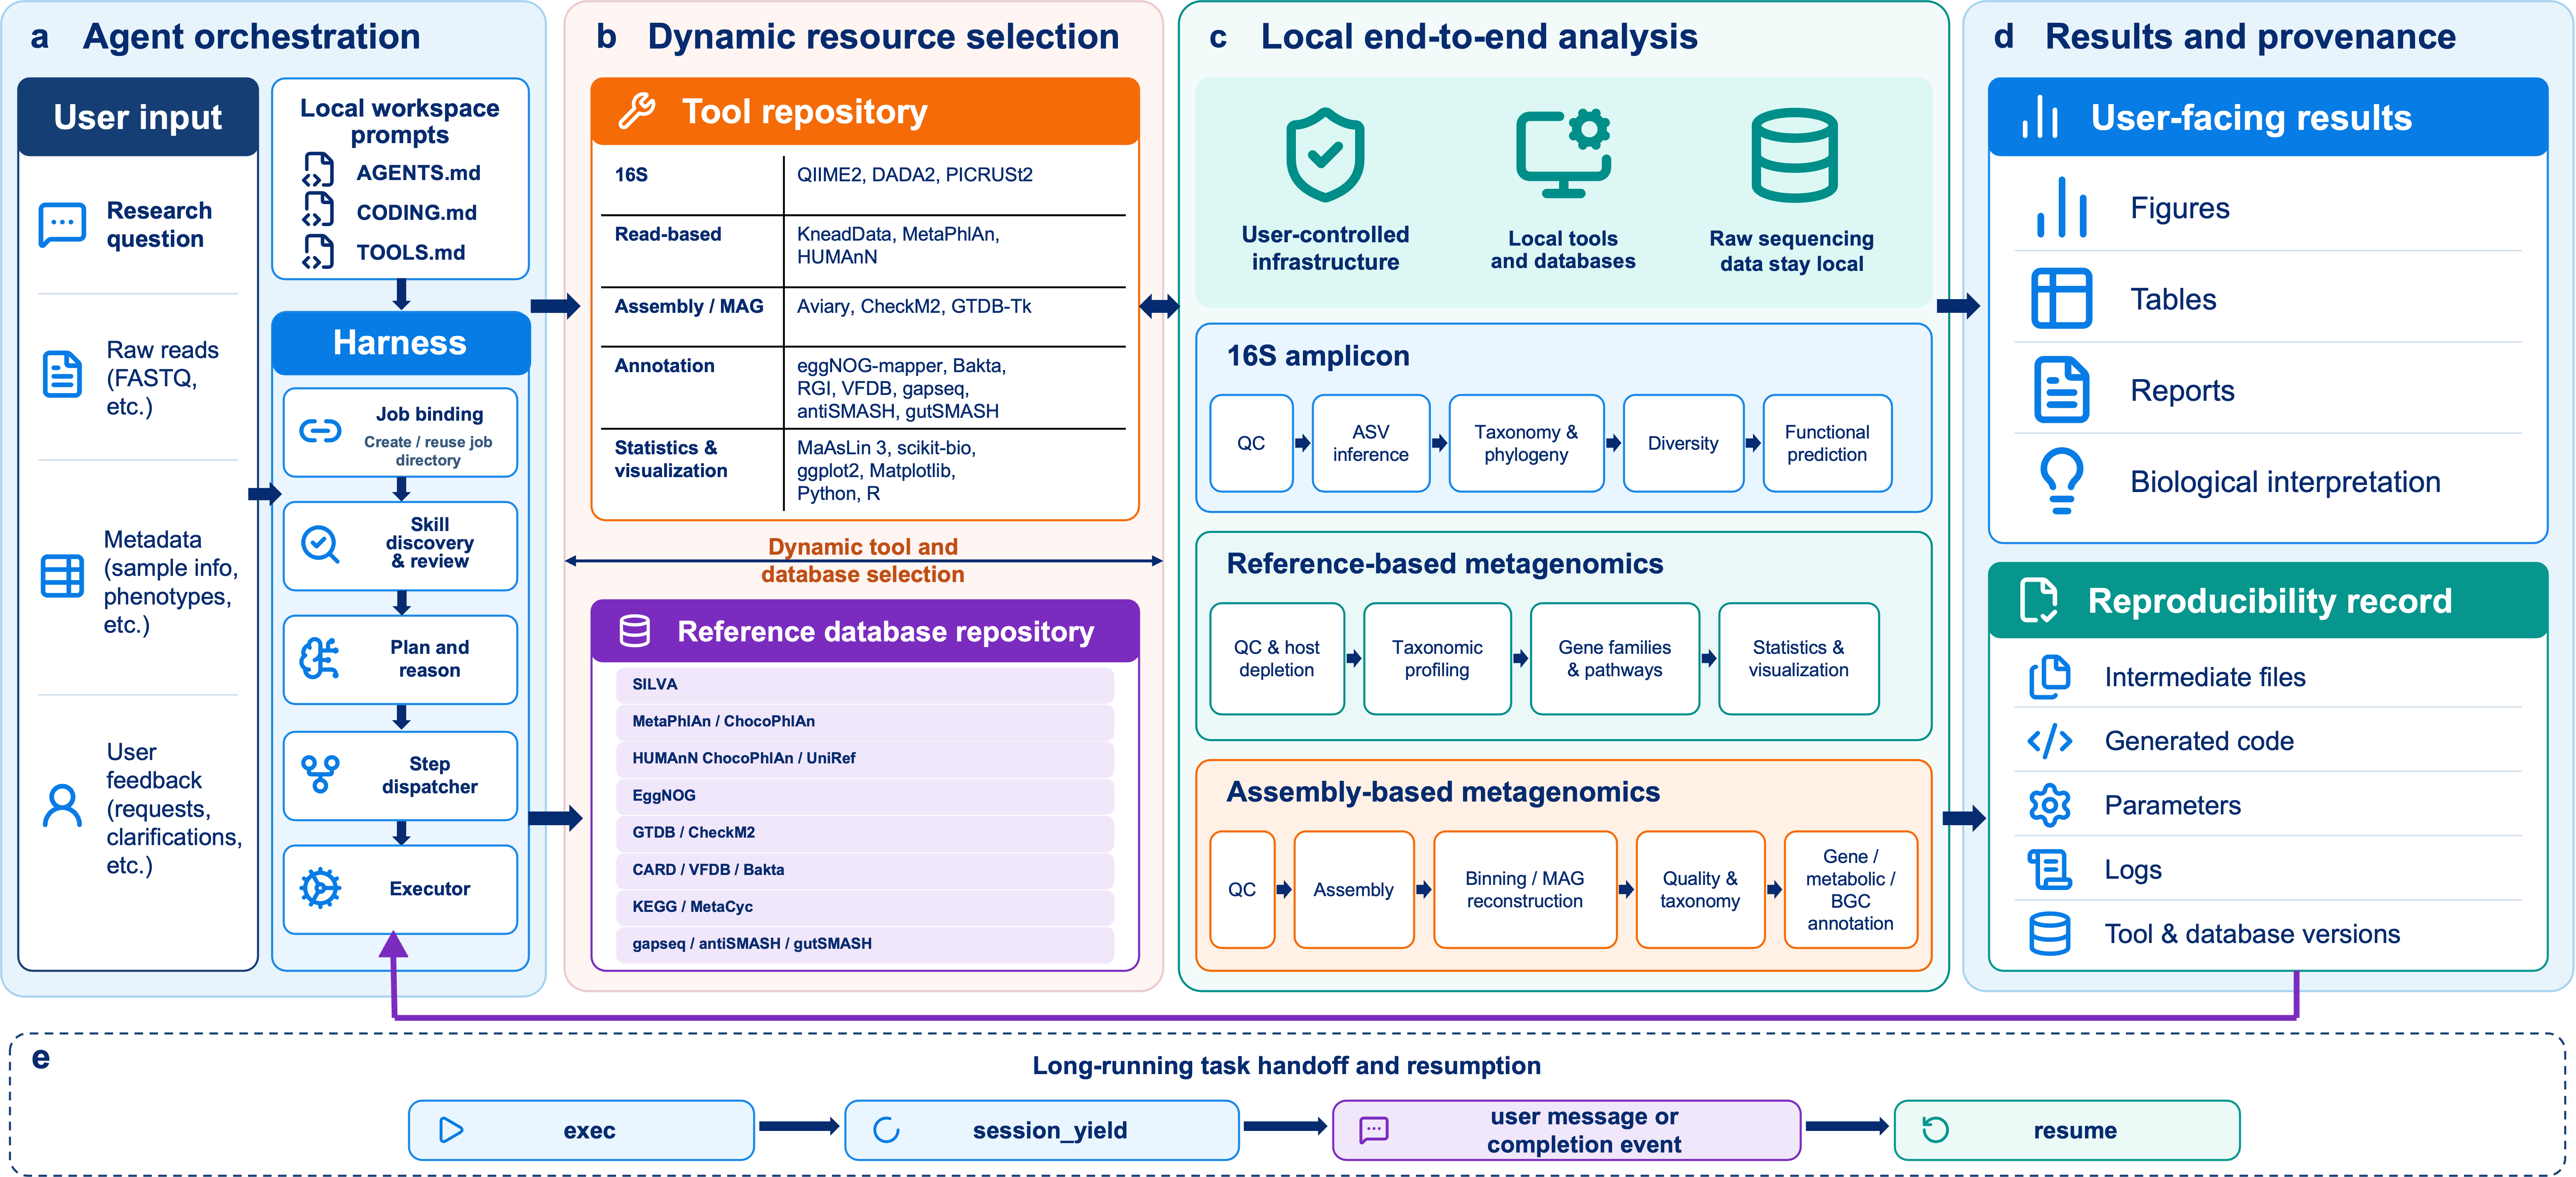
\includegraphics[width=\linewidth]{microbioagent-architecture-image2-v7.png}
  \caption{MicroBioAgent architecture and operating model.  A user request is
    bound to an analysis job, from which the agent plans, selects skills, and
    resolves local runtimes and reference resources for 16S amplicon,
    reference-based shotgun, and assembly-based metagenomic analyses.
    Intermediate artifacts, commands, parameters, and logs remain associated
    with the job.  During long-running computation, a user message can update
    pending work, whereas command completion triggers output verification and
    continuation in the same session.}
  \label{fig:architecture}
\end{figure}

MicroBioAgent is an AI-agent framework that integrates flexible composition
of upstream and downstream microbiome analyses, local execution, and
asynchronous human-in-the-loop interaction (\cref{fig:architecture}).
Given a research question expressed in natural language, it develops an
analysis plan and selects microbiome skills to carry it out.  These
skills provide method-specific guidance that the agent draws on when choosing
analytical approaches, preparing commands, and interpreting outputs.  As each
step completes, the agent examines its results and decides whether the pending
plan needs adjustment.

MicroBioAgent executes upstream processing and downstream analyses in a
user-controlled local computational environment, without requiring raw
sequencing data to be uploaded to an external analysis platform.  To support
these analyses, the system manages analytical tools and reference databases
through separate configuration files.  The tool configuration specifies
available software and its associated execution environments, while the
database configuration records reference resources and their local storage
paths.  Users can modify these configurations to add or replace tools and
reference databases according to their research needs.

For upstream analysis, MicroBioAgent supports 16S amplicon processing,
reference-based metagenomic profiling, and assembly-based metagenomic
reconstruction (\cref{tab:skills}).  Its amplicon capabilities include sequence
quality assessment, denoising, amplicon sequence variant inference, taxonomic
classification, and phylogenetic reconstruction.  For shotgun data, it supports
read quality control and host-read removal, taxonomic and functional profiling,
and gene-catalogue construction.  Assembly-based capabilities include
metagenomic assembly and binning, MAG quality assessment, dereplication,
taxonomic assignment, and abundance estimation.

MicroBioAgent supports a range of downstream analyses, such as comparisons of
microbial communities and characterization of the functions of individual
organisms.  These include comparisons of diversity and taxonomic or functional
abundances between groups, covariate association testing, functional enrichment,
association network analysis, and supervised classification.
For genes and recovered genomes, available
analyses include functional and pathway annotation, antimicrobial-resistance
and virulence-gene annotation, metabolic reconstruction, and identification of
primary metabolic and secondary-metabolite biosynthetic gene clusters.
For visualization, MicroBioAgent supports ordination plots of community
differences and heatmaps of taxonomic abundances or functional profiles,
with customization to highlight the comparisons of interest.

During long-running computations, such as MetaPhlAn or HUMAnN profiling,
MicroBioAgent keeps the conversation available for user interaction while the
analysis runs in the background.  Users can provide additional instructions or
revise the pending analysis plan without waiting for the running task to finish.
This asynchronous human-in-the-loop interaction allows the agent to incorporate
feedback during execution and automatically resume the analysis under the
updated plan after checking the completed task's outcome.  MicroBioAgent thus
supports end-to-end microbiome analysis through flexible workflow composition
and local execution, while allowing users to guide ongoing analyses.

\begin{table}[!htbp]
  \centering
  \caption{MicroBioAgent analytical capabilities, grouped by scientific task.
    Functional predictions and genome annotations describe inferred biological
    potential.}
  \label{tab:skills}
  \small
  \renewcommand{\arraystretch}{1.12}
  \begin{tabularx}{\linewidth}{@{}>{\raggedright\arraybackslash}p{0.25\linewidth}>{\raggedright\arraybackslash}X@{}}
    \toprule
    Task category & Supported analyses \\
    \midrule
    Amplicon characterization
      & Read import and quality summaries, denoising and ASV inference,
        taxonomy, phylogeny, predicted functional profiles \\
    Shotgun profiling
      & Read quality control and host depletion, species abundances,
        gene-family and pathway profiles, nonredundant gene catalogues \\
    MAG characterization
      & Assembly and binning, quality assessment.  Dereplication,
        taxonomic assignment, abundance estimation, genome annotation \\
    Community comparisons
      & Alpha and beta diversity, ordination, group comparisons,
        differential abundance, covariate association testing \\
    Functional interpretation
      & Gene and protein annotation, orthology, pathway, and ontology mapping,
        functional enrichment, resistance and virulence gene annotation \\
    Metabolic characterization
      & Metabolic pathway and model reconstruction, primary metabolic gene
        clusters, secondary-metabolite biosynthetic gene clusters \\
    Study-specific analysis
      & Custom statistical scripts, association networks, supervised
        classification, figures, result tables, and analytical reports \\
    Data and resource access
      & Public sequencing metadata and reference-protein retrieval,
        local reference resources and online annotation queries \\
    \bottomrule
  \end{tabularx}
\end{table}

\subsection{Study-specific analyses across plant, human, and environmental microbiomes}
\label{sec:case-studies}

We evaluated MicroBioAgent on three published datasets comprising 230
sequencing libraries from plant, human, and environmental microbiomes
(Supplementary Table~\ref{tab:cases-overview}).  These case studies assessed
the system's ability to complete the requested analyses and recover biological
patterns reported in the source studies.  Because software versions, reference
databases, and some statistical procedures differed, exact computational
reproduction was not the evaluation objective.  Instead, we assessed completion
of the requested analyses, validity of the resulting outputs, and recovery of
prespecified biological signals.

The three cases were selected to test MicroBioAgent on distinct combinations
of data types and analytical tasks.  The tomato rhizosphere case combined 60
16S amplicon libraries with 36 matched shotgun libraries to examine differences
in microbial diversity and taxonomic composition associated with pathogen
inoculation and cultivar resistance.  The colorectal cancer case used 128
faecal shotgun metagenomes from 74 patients and 54 controls to compare species
and functional abundances and train classifiers based on gene-family and KEGG
Orthology profiles.  The third case used six shotgun metagenomes from
soil-derived enrichment cultures grown on low-molecular-weight polyethylene or
alkane substrates to generate MAGs through assembly and binning, dereplicate
them, characterize their taxonomic composition, and annotate
degradation-associated genes in focal genomes.

\subsubsection{A tomato rhizosphere bacterial-wilt resistance study}
\label{sec:case-tomato}

We applied MicroBioAgent to a published study of tomato rhizosphere
microbiomes associated with resistance to bacterial wilt
\parencite{yin2022tomato}.  This case evaluated its ability to connect
amplicon and shotgun analyses to examine resistance-associated community
changes and identify the species markers reported in that study.
The input comprised 60 16S V3--V4 amplicon
libraries and 36 matched shotgun libraries from two susceptible cultivars
(A57 and HG70), a resistant parent (HG64), and a resistant F1 hybrid (HF12).
The amplicon data covered five sampling conditions with three biological
replicates per cultivar, including before inoculation (T1), and inoculated and
uninoculated plants at day 5 (T2 and T2C) and day 10 (T3 and T3C).
The matched shotgun libraries covered T1, T2C, and T2.
Starting from sequencing reads, MicroBioAgent performed quality control,
DADA2 denoising and taxonomic classification against the SILVA database for
the amplicon data, and quality control, host-read removal and MetaPhlAn3
taxonomic profiling for the shotgun data.  The resulting profiles supported
community-level comparisons using 16S data and species-level marker analysis
using shotgun data.

For the 16S amplicon data, MicroBioAgent examined how pathogen inoculation
and cultivar resistance were reflected in microbial diversity and community
composition.  Following \textit{Ralstonia} inoculation, Shannon diversity
declined in susceptible cultivars and remained higher in resistant cultivars
at both day 5 ($P=0.002$) and day 10 ($P=0.004$,
\cref{fig:tomato-diversity}a).  Community composition also differed between inoculated and uninoculated
samples, which separated along the first weighted-UniFrac PCoA axis
(56.3\% of variance).  Resistant and susceptible samples showed a less
pronounced separation along the second axis (12.2\%), with overlap between
the two groups (\cref{fig:tomato-diversity}b).  Genus-level profiles linked these community
changes to an expansion of \textit{Ralstonia}, most pronounced in the
susceptible cultivars A57 and HG70 (\cref{fig:tomato-diversity}c).
These patterns were consistent with the inoculation-associated community
changes and higher post-inoculation diversity in resistant cultivars
reported in the source study.

To examine the taxa underlying these resistance-associated differences,
MicroBioAgent compared each resistant cultivar with the pooled susceptible
cultivars using MaAsLin~3.  In the 16S profiles, the number of genera
enriched in both HG64 and HF12 ranged from 6 to 15 across sampling
conditions, with different genera contributing to these shared enrichments
(Supplementary Figure~\ref{fig:tomato-enrichment}).  The matched shotgun data provided species-level
comparisons of the markers highlighted in the source study.  MetaPhlAn3
profiles showed enrichment of the \textit{Pseudomonas putida} group in both
the resistant parent HG64 ($P=0.013$) and the resistant hybrid HF12
($P=0.009$) at T1.  The other reported marker,
\textit{Sphingopyxis unclassified}, was not identified in the MetaPhlAn3
profiles.  Following investigator review, MicroBioAgent repeated the shotgun
profiling using MetaPhlAn2, the version used in the original study, and
identified both \textit{Pseudomonas putida} and \textit{Sphingopyxis unclassified}
as enriched in resistant cultivars, recovering both reported taxonomic
associations.
% SUPPLEMENTARY PLACEHOLDER: case1-metaphlan-version-sensitivity
% SUPPLEMENTARY PLACEHOLDER: case1-16s-statistics

\begin{figure}[htbp]
  \centering
  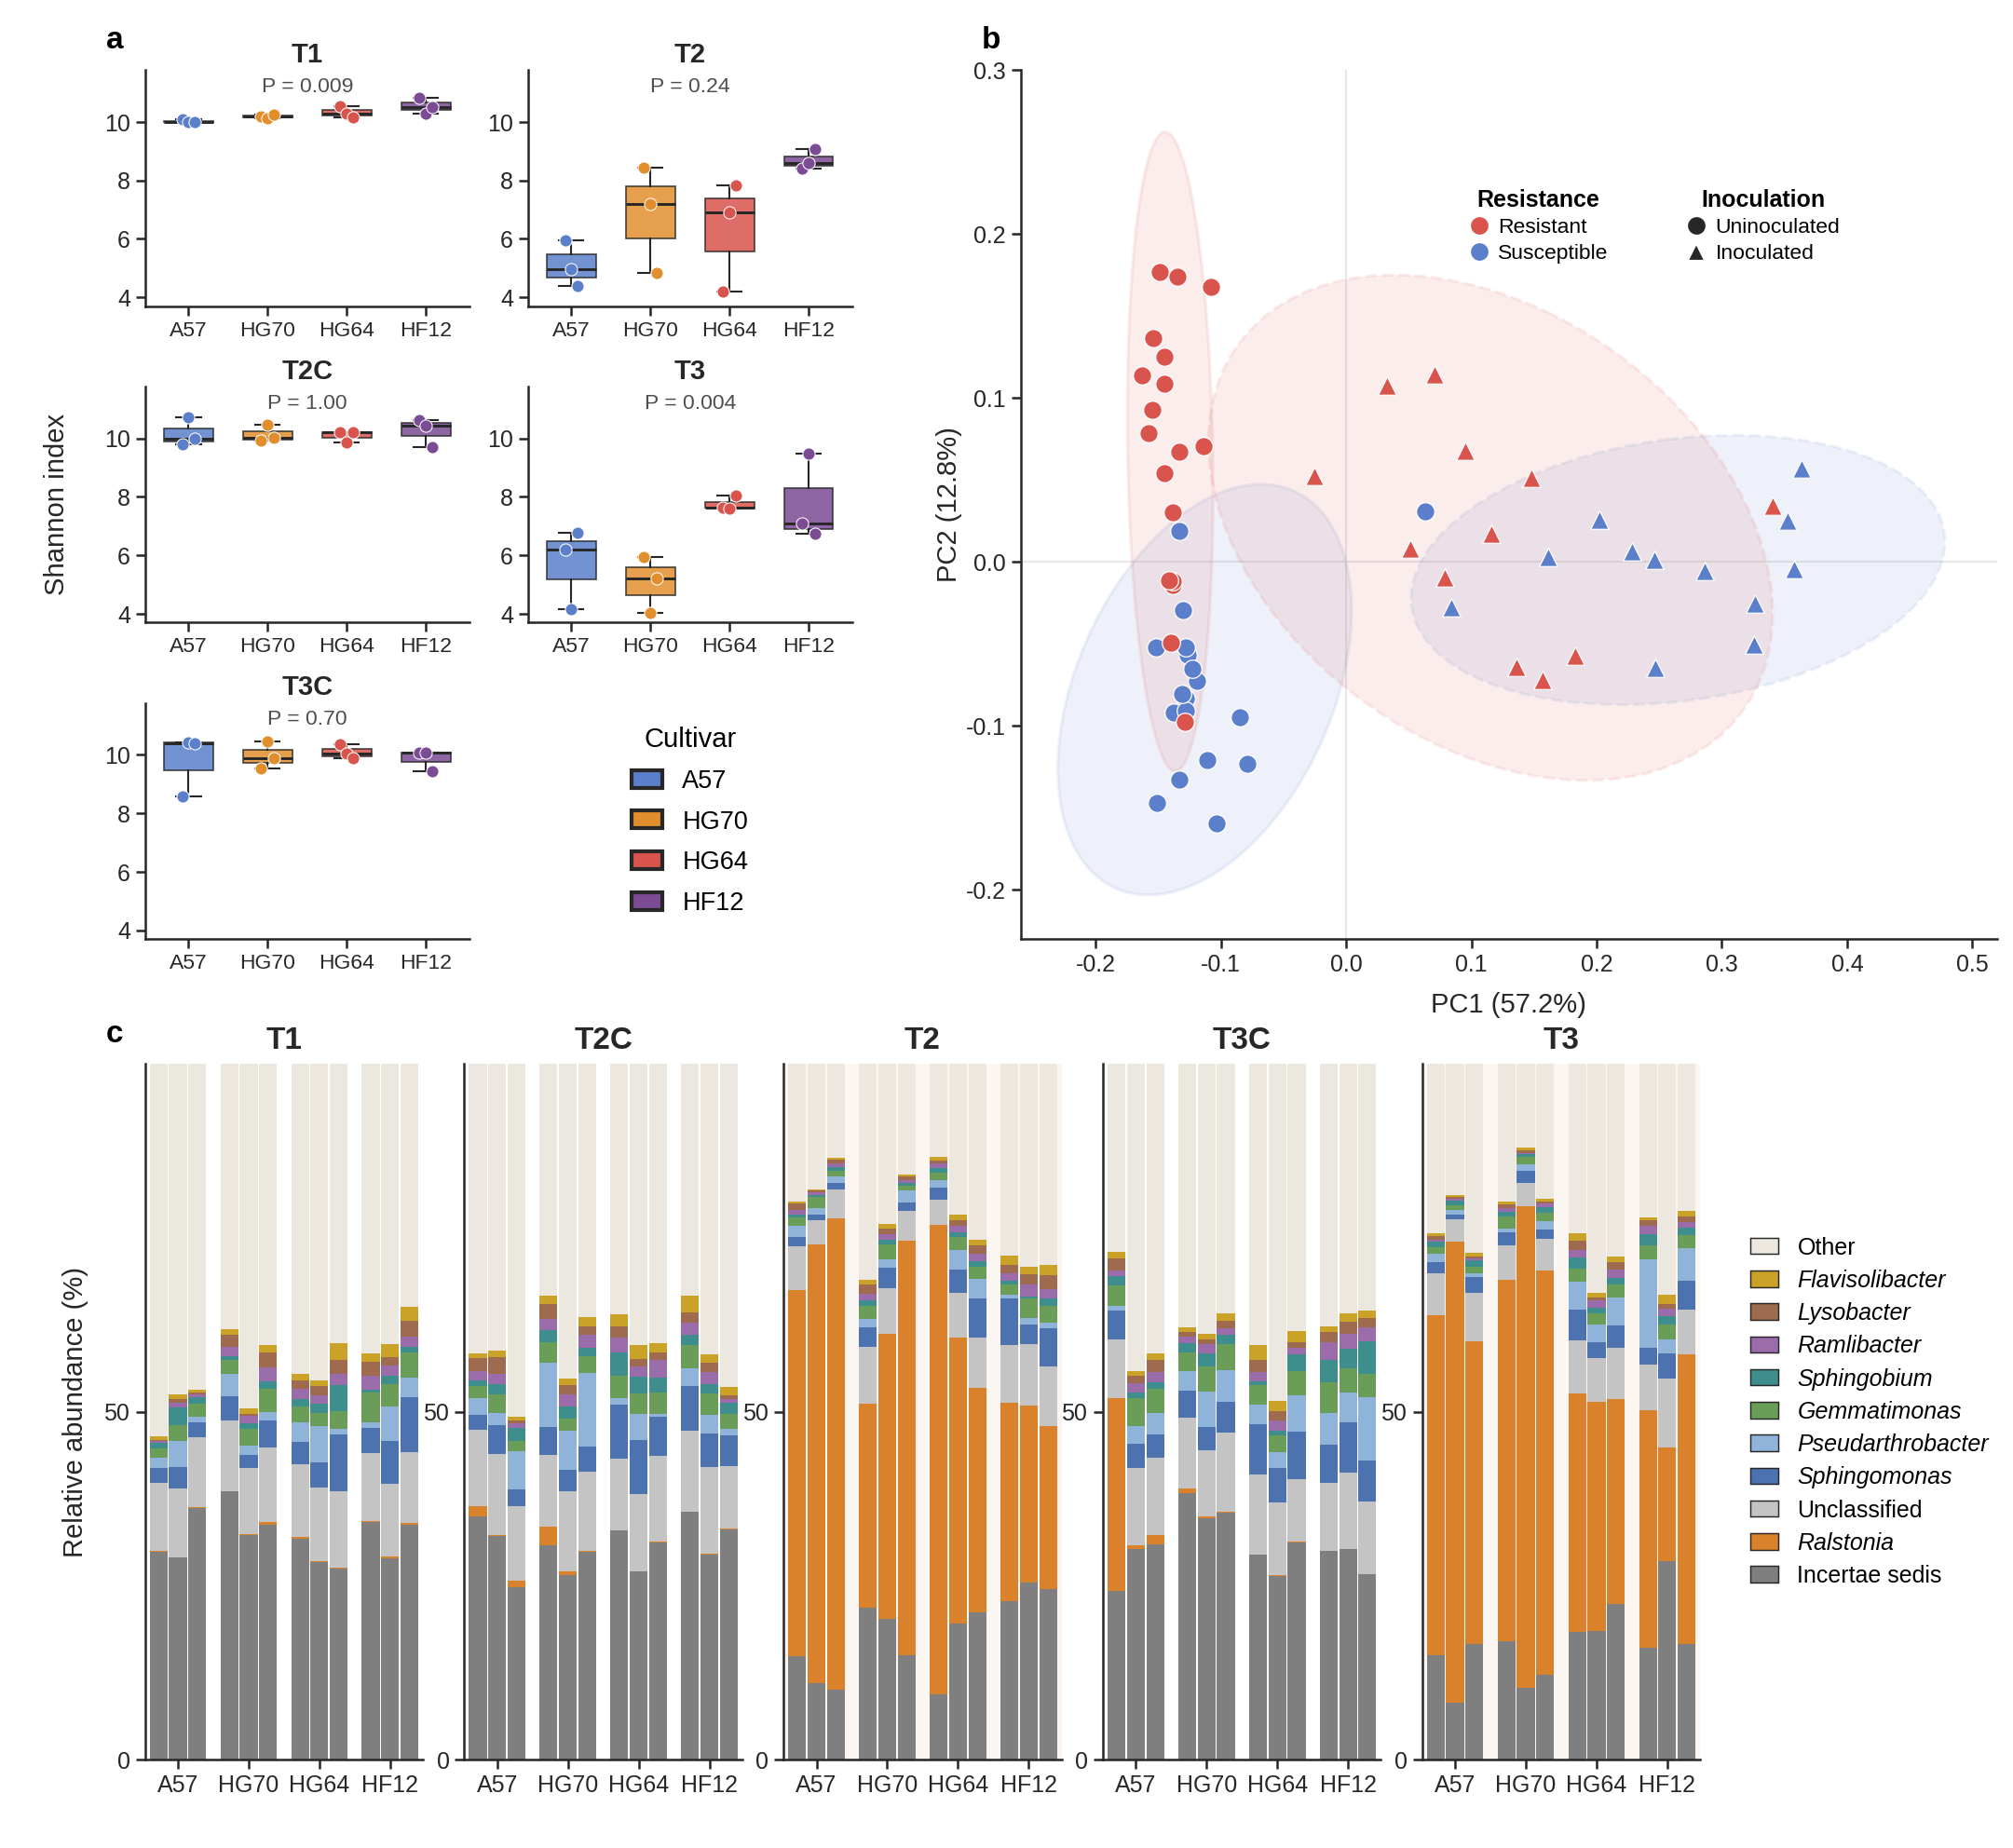
\includegraphics[width=0.94\linewidth]{Case-study-1-Fig1_diversity.png}
  \caption{Tomato rhizosphere diversity and community composition.  (a)
    Shannon diversity across cultivars, sampling time points, and inoculation
    conditions.  (b) Weighted-UniFrac PCoA, coloured by resistance phenotype
    and shaped by inoculation treatment.  (c) Genus-level composition across
    individual samples.  Each cultivar-time-point combination contained three
    biological replicates.}
  \label{fig:tomato-diversity}
\end{figure}



% Keep the tomato diversity figure with Case 1.
\FloatBarrier

\subsubsection{A colorectal cancer faecal metagenomic biomarker study}
\label{sec:case-crc}

The colorectal cancer (CRC) case evaluated whether MicroBioAgent could
connect taxonomic and functional profiling to disease-associated species
analysis, co-occurrence networks and predictive modelling.
The dataset comprised 128 faecal metagenomes from the Hong Kong
C1 cohort reported by Yu \textit{et al.}, including 74 patients with CRC
and 54 controls \parencite{yu2017crc}.  MicroBioAgent performed species-level
profiling with MetaPhlAn3 and quantified UniRef90 gene-family and KEGG
Orthology (KO) abundances with HUMAnN3 for downstream association analysis
and classification (\cref{fig:crc}).  Reported species associations and
co-occurrence patterns provided biological reference points, while
cross-validation assessed the predictive performance of the functional
features.

PCoA based on Bray--Curtis dissimilarities calculated from MetaPhlAn3
species-level relative abundance profiles showed no clear separation
among controls, early-stage CRC cases ($n=36$) and late-stage CRC cases
($n=38$).  PERMANOVA nevertheless detected differences in community
composition associated with CRC status ($F=2.32$, $P=0.002$) and disease
stage ($F=1.65$, $P=0.009$).  Separate tests for sex, age and BMI were
not significant.

Comparisons of species abundances between cases and controls identified
eight CRC-enriched and two control-enriched taxa after Benjamini--Hochberg
correction ($q<0.05$).  Four CRC-enriched species,
\textit{Parvimonas micra}, \textit{Peptostreptococcus stomatis},
\textit{Fusobacterium nucleatum} and \textit{Solobacterium moorei}, showed
the same direction of association as in the original study.  Enrichment
of \textit{Eubacterium ventriosum} in controls also agreed with the
reported association.  To examine whether these disease-associated species
also varied together across samples, Spearman co-occurrence analysis was
performed on the ten differentially abundant species.  The network contained
16 positive correlations ($|\rho|\geq0.4$, BH-adjusted $q<0.05$), with
\textit{Parvimonas micra} connected to six other species.
Its positive correlations with \textit{Fusobacterium nucleatum}
($\rho=0.49$) and \textit{Solobacterium moorei} ($\rho=0.53$) were
consistent with the co-occurrence relationships emphasized in the original
study \parencite{yu2017crc}.

The analysis then extended from identifying disease-associated taxa to
testing whether functional differences could distinguish CRC cases from
controls.  MicroBioAgent selected differentially abundant features and
trained separate gene-family and KO classifiers to compare the predictive
performance of these two functional representations.  Within each training fold,
mRMR selection yielded 15 gene-family features or 15 KO features for
logistic-regression modelling.  Performance was evaluated by nested
fivefold cross-validation within the C1 cohort.  The gene-family
classifier achieved a pooled out-of-fold AUROC of 0.902, compared with
0.632 for the KO classifier, indicating stronger discrimination using
gene-family features.  At thresholds selected using Youden's index,
the gene-family classifier achieved a sensitivity of 0.82 and specificity
of 0.89, compared with 0.41 and 0.87 for the KO classifier.
% SUPPLEMENTARY PLACEHOLDER: case3-species-and-function-tests
% SUPPLEMENTARY PLACEHOLDER: case3-classifier-folds
% Outer-fold AUROC ranges: gene-family 0.86--0.96, KO 0.59--0.72.
% Include these values and per-fold results in the supplementary classifier table.

\begin{figure}[htbp]
  \centering
  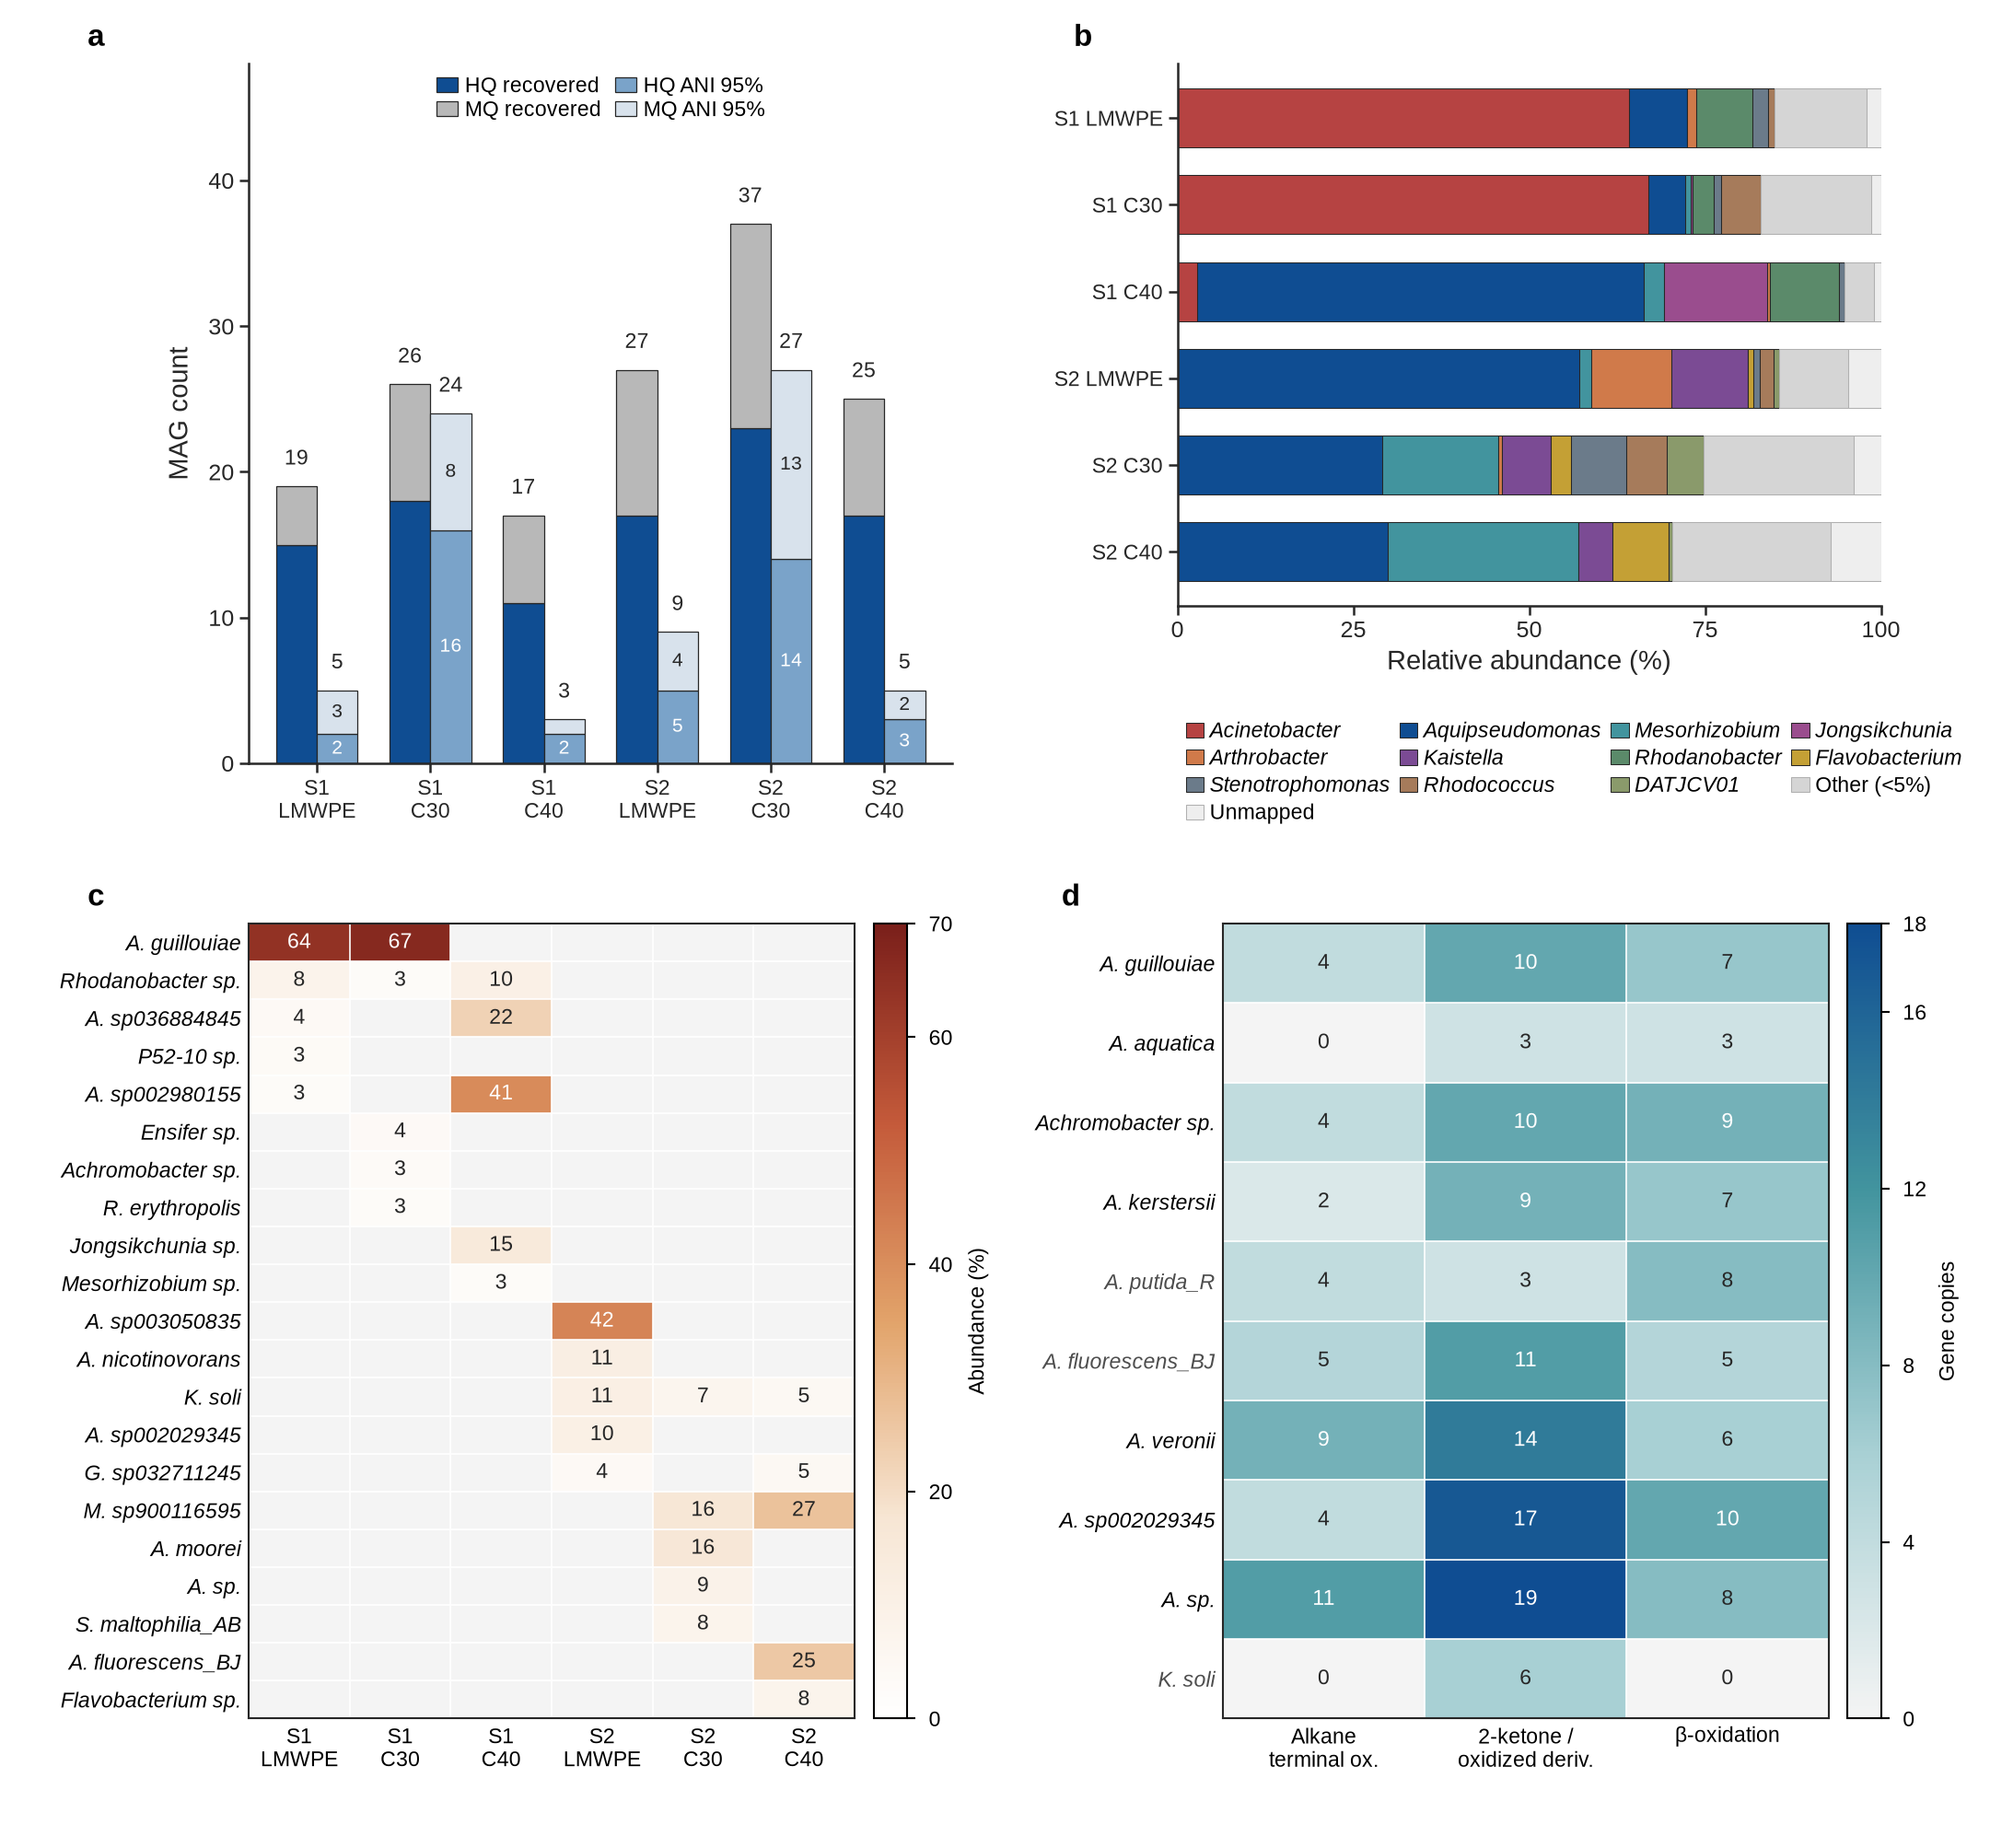
\includegraphics[width=0.94\linewidth]{Case-study-3-Fig_composite.png}
  \caption{Reference-based analysis of CRC faecal metagenomes.  Species-level
    beta diversity, disease-associated taxa, co-occurrence of the
    differentially abundant species, functional features, and nested
    cross-validation of gene-family and KO classifiers are shown.}
  \label{fig:crc}
\end{figure}

\FloatBarrier

\subsubsection{A polyethylene-enrichment genome-resolved metagenomic study}
\label{sec:case-mag}

We next evaluated whether MicroBioAgent could reconstruct genomes from
enrichment metagenomes and use them to identify microorganisms and annotate
genes associated with alkane and oxidized-derivative metabolism.
The dataset comprised six Oxford Nanopore long-read metagenomes from two
soil inocula (S1 and S2), each enriched on low-molecular-weight polyethylene
(LMWPE), triacontane (C30) or tetracontane (C40)
\parencite{sandholm2025polyethylene}.  Assembly and binning generated
372 bins, of which 153 passed completeness and contamination filtering
(100 high-quality and 53 medium-quality MAGs).
Dereplication at 95\% average nucleotide identity retained 75 representative
genomes (50 high quality and 25 medium quality, \cref{fig:mag}a).
These genomes were classified using GTDB-Tk with GTDB release R232,
and their abundances across the enrichment cultures were estimated by
read mapping with CoverM to identify the predominant microorganisms in
each enrichment culture.

MAG abundance profiles showed different dominant taxa across the enrichment
cultures.  \textit{Acinetobacter guillouiae} dominated S1 LMWPE and S1 C30,
accounting for 64\% and 67\% of the reported abundance, respectively.
S1 C40 was instead dominated by \textit{Aquipseudomonas}, which accounted
for 66\% at the genus level (\cref{fig:mag}b,c).  The S2 cultures showed
a different composition.  \textit{Aquipseudomonas} sp003050835 was most
abundant in S2 LMWPE (42\%), while \textit{Mesorhizobium\_M} sp900116595
and \textit{Aquipseudomonas moorei} were the most abundant species in
S2 C30 (16\% each).  In S2 C40, \textit{Mesorhizobium\_M} sp900116595
and \textit{Aquipseudomonas fluorescens\_BJ} predominated at 27\% and
25\%, respectively.  Taxonomic annotation identified the ten taxonomic groups of particular
interest in the original study
(Supplementary Table~\ref{tab:mag-taxonomy}).  The groups reported as
\textit{Pseudomonas} in the original study were classified as
\textit{Aquipseudomonas} in the present analysis due to differences
in the reference taxonomy.

To examine the metabolic potential of the ten taxonomic groups emphasized
in the original study, functional annotation was performed on one
representative MAG from each group.
The annotations identified genes associated with the three metabolic
processes examined in the original study (\cref{fig:mag}d).
Genes associated with alkane terminal oxidation
were annotated in eight MAGs, while those associated with 2-ketone or
oxidized-derivative metabolism were detected in all ten.  Nine MAGs
contained genes assigned to the $\beta$-oxidation module M00087.
Eight MAGs contained annotations spanning all three categories,
indicating that the corresponding genetic potential was distributed
across multiple taxa of interest.
% SUPPLEMENTARY PLACEHOLDER: case4-mag-catalogue
% SUPPLEMENTARY PLACEHOLDER: case4-functional-annotations
% SUPPLEMENTARY PLACEHOLDER: case4-mag-taxonomy (Table~\ref{tab:mag-taxonomy})
% Populate with MAG identifiers and current GTDB assignments from the annotation
% export. Confirm whether it covers all 153 quality-filtered MAGs or only the
% 75 dereplicated representatives before specifying the table's MAG count.

\begin{figure}[htbp]
  \centering
  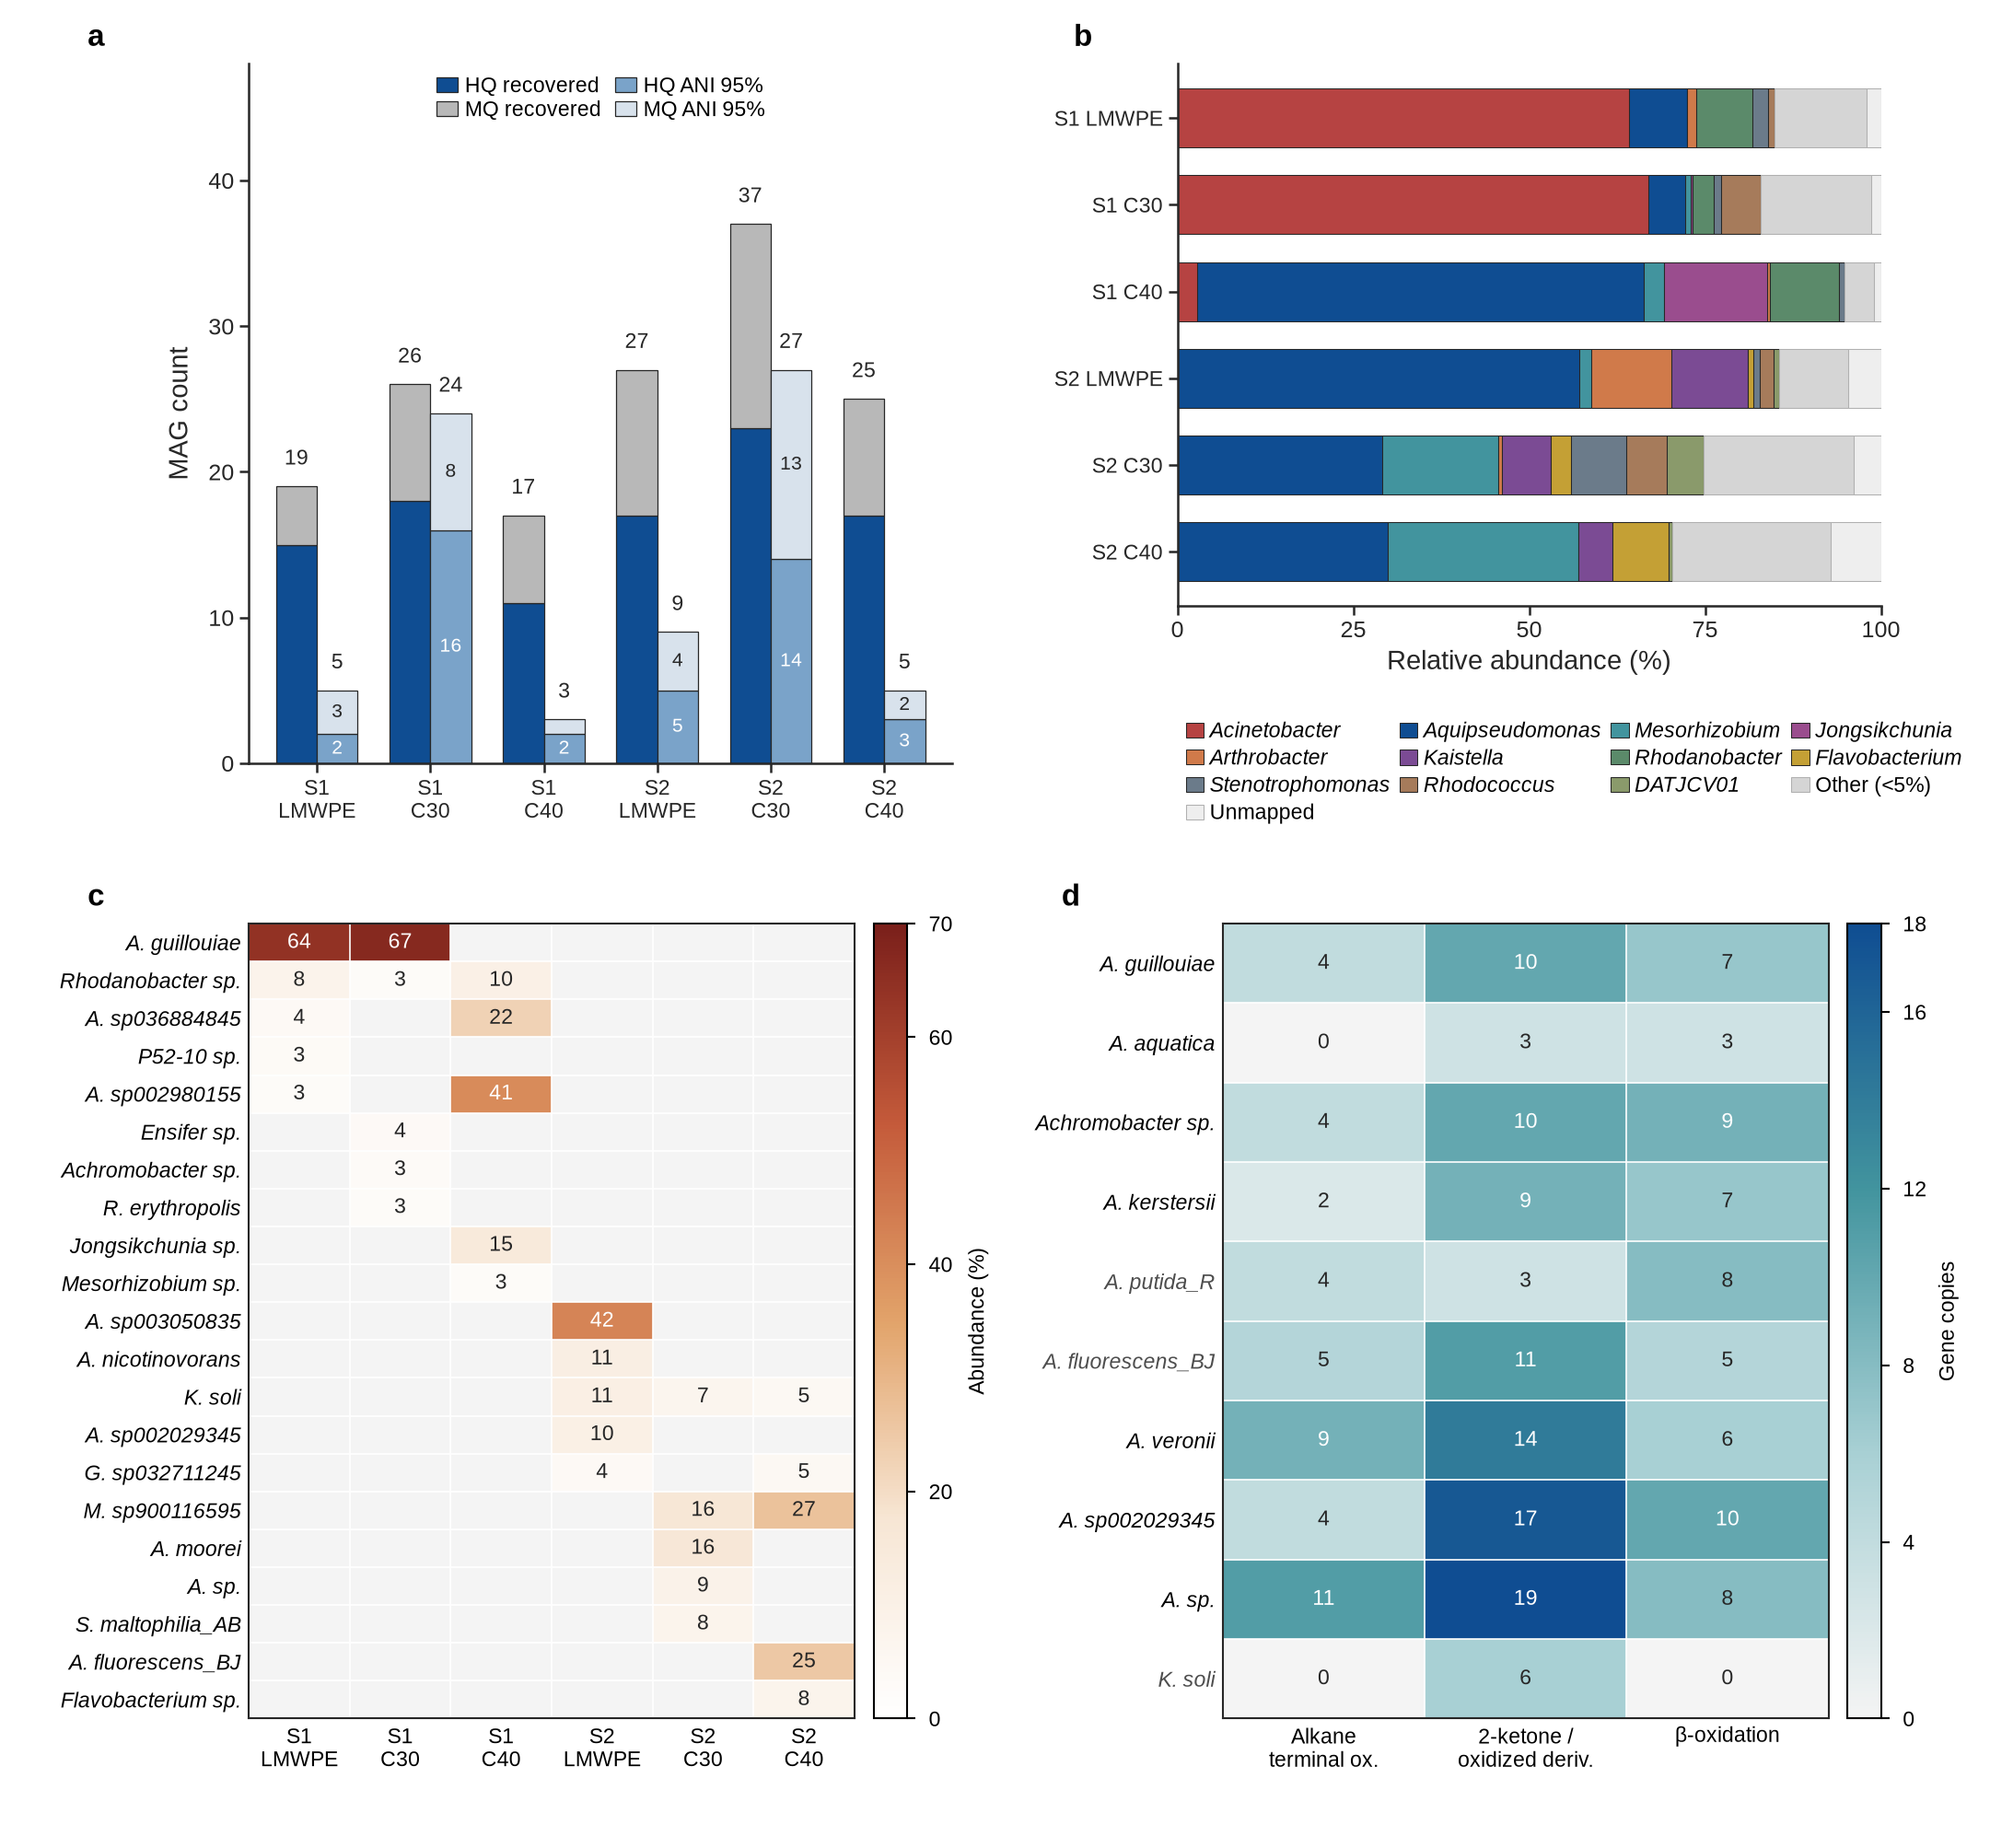
\includegraphics[width=0.94\linewidth]{Case-study-4-Fig_composite.png}
  \caption{Assembly-based analysis of enrichment metagenomes.  (a) Numbers of
    high- and medium-quality MAGs, grouped by completeness and contamination
    thresholds defined in Methods, before and after 95\% ANI dereplication.
    (b) Genus-level MAG composition.  (c) Species among the five most abundant
    MAGs in at least one sample.  (d) Numbers of genes annotated using
    eggNOG-mapper in one representative MAG per target taxon for alkane
    terminal oxidation, 2-ketone or oxidized-derivative metabolism, and
    $\beta$-oxidation (M00087).  Counts represent annotated genes rather
    than distinct functional types or transcript abundance.}
  \label{fig:mag}
\end{figure}

\FloatBarrier

\subsection{Robustness across models and prompt granularity}
\label{sec:robustness}

We evaluated completion and output stability on the frozen Case~1 inputs
with the complete system.  Three models, DeepSeek-Pro, DeepSeek-Flash and
GLM-Flash, were crossed with detailed, medium and simple prompts, and each
cell contained three sessions.  Six analyses were scored: 16S alpha
diversity, 16S beta diversity, 16S taxonomic profiling, 16S differential
abundance, shotgun species-level taxonomic profiling and shotgun
differential abundance (Supplementary Figure~\ref{fig:robustness-models}a).
Every 16S analysis was completed in three of three sessions.  Shotgun
taxonomic profiling and shotgun differential abundance were likewise
completed in three of three sessions, except under the GLM-Flash detailed
prompt (2/3), where one session contained no shotgun reads.

Shannon index, pairwise weighted UniFrac distance and DESeq2 log$_2$ fold
change did not differ among models (Supplementary
Figure~\ref{fig:robustness-models}b).  For both diversity summaries, every
model pair had a Holm-adjusted $P = 1$ within each prompt.  DESeq2
comparisons used only sessions that ran DESeq2 and only taxa shared across
those sessions (Supplementary Table~\ref{tab:da-model-methods}): 216 genera
for the detailed 16S prompt, 332 genera for the medium 16S prompt and 43
species for the detailed shotgun prompt.  No model pair differed after Holm
correction.  The medium shotgun prompt yielded no DESeq2 results that could
be compared across models, and DeepSeek-Pro contributed one of three
sessions to each DESeq2 comparison.  Relative abundance of shared genera
and species differed among models in some prompt conditions.

Within each model, prompt level left the Shannon index and weighted UniFrac
distance unchanged (Supplementary Figure~\ref{fig:robustness-prompts}).
Relative abundance differed between some prompt levels.  Detailed and medium
16S analyses both used DESeq2.  Their genus-level log$_2$ fold changes
differed for DeepSeek-Pro (111 shared genera, $P = 0.014$) and did not
differ for DeepSeek-Flash (668 genera, $P = 0.32$) or GLM-Flash (413 genera,
$P = 0.28$).  Shotgun detailed-versus-medium contrasts were not significant
within any model ($P = 0.16$, $0.73$ and $0.25$ for DeepSeek-Pro,
DeepSeek-Flash and GLM-Flash).  These shotgun values are not the same
estimand: DeepSeek-Pro reported a Wilcoxon log$_2$ fold change,
DeepSeek-Flash a Mann--Whitney $U$ log$_2$ fold change and GLM-Flash a
DESeq2 log$_2$ fold change (Supplementary Table~\ref{tab:da-prompt-methods}).
They were therefore not compared across models.

The rank tests compare distributions of magnitudes.  Samples, sample pairs
and taxa come from this one experiment and are not independent replicates.
The comparisons do not establish that community structure was preserved or
that the same taxa were called as differentially abundant.

\FloatBarrier

\subsection{Evaluating component contributions and asynchronous guidance}
\label{sec:ablation}

\subsubsection{Component contributions to end-to-end analysis}

We compared the complete system with removal of the shipped microbiome skills
and with removal of the coding and long-execution instructions
(\cref{fig:component-ablation}).  The session-runtime extension was left in
place.  Every condition used the detailed Case~1 prompt, the frozen
preprocessed inputs, and one model, with no user message after the initial
plan confirmation.  The complete-system sessions are the three detailed-prompt
\texttt{deepseek-v4-pro} sessions.  Each ablated condition was scored from
three archived sessions.

All nine requested outputs were present in each complete-system session.
Without skills, one session did not contain an analysis report (26 of 27
output checks).  Without coding guidance, one session did not retain analysis
scripts (26 of 27 output checks); the other requested outputs were present.
All eight methods named in the detailed prompt were used in every session.
Token totals were not present in the archived job records.

This comparison asks whether those components were required to finish the
prespecified downstream analysis when the prompt already named the methods.
It does not test upstream read processing, other models, or less specific
prompts.

\begin{figure}[htbp]
  \centering
  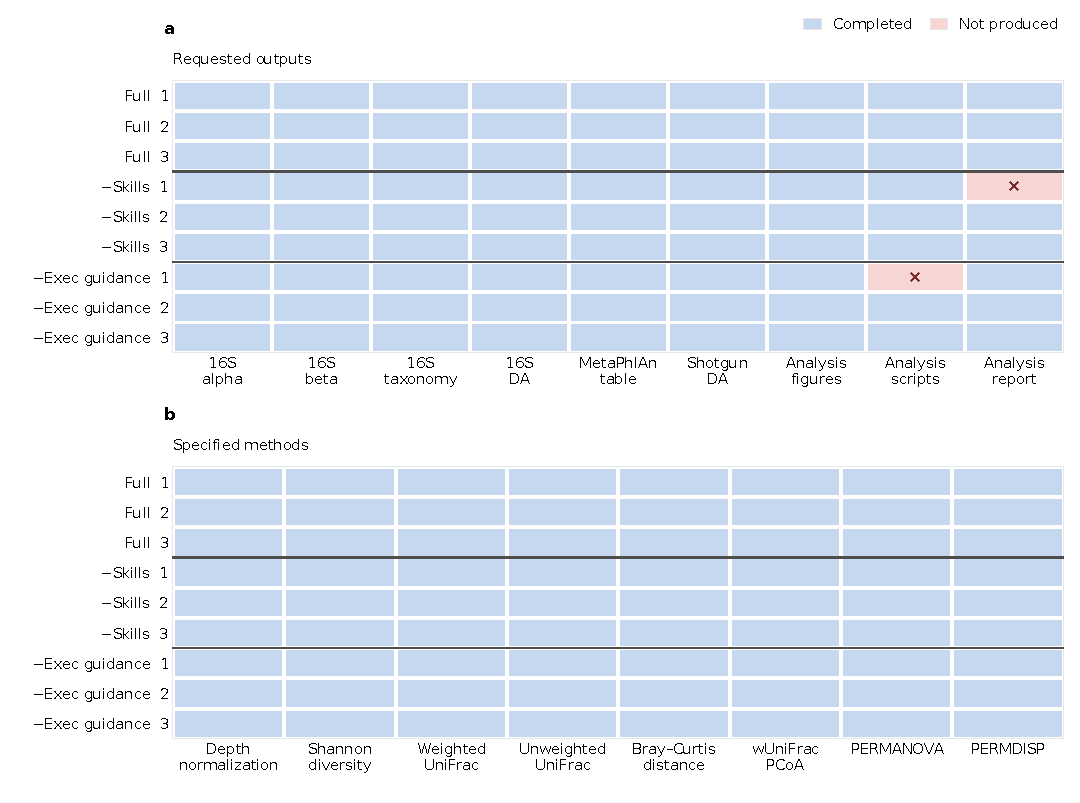
\includegraphics[width=\linewidth]{component_ablation.pdf}
  \caption{Component contributions to end-to-end Case~1 analysis.
    (a)~Nine requested outputs.
    (b)~Eight methods named in the detailed prompt: sequencing-depth
    normalization, Shannon diversity, weighted UniFrac, unweighted UniFrac,
    Bray--Curtis distance, weighted-UniFrac PCoA, PERMANOVA, and PERMDISP.
    Each row is one independent session.
    A cell is filled when that output or method was present in the archived
    job and marked when it was not.
    Full is the complete system, $-$Skills removes the microbiome domain
    skills, and $-$Exec guidance removes the coding and long-execution
    instructions.
    Each condition contains three sessions.
    Completion records whether a usable artifact was produced.
    It is not a test of agreement with the original study.}
  \label{fig:component-ablation}
\end{figure}

\subsubsection{Runtime ablation for analysis continuity}

We tested asynchronous guidance with a real, minutes-scale Case~1 QIIME~2
taxonomy-classification task.  After the command was confirmed running, the
user instructed the agent to replace a pooled resistant-versus-susceptible
comparison with separate T1, T2C, and T2 comparisons and to add a
significant-genera heatmap.  No subsequent ``continue'' message was sent.

With the extended runtime, the agent yielded while the command continued,
updated the pending plan during execution, and resumed automatically after
command completion in all three sessions (\cref{tab:hitl-ablation}).  With
the standard runtime in the tested configuration, neither plan revision during
active computation nor automatic session resumption after tool exit was
observed in any of the three sessions.
These observations support plan revision and automatic continuation for the
tested command and runtime configuration.  The two endpoints assess session
interaction.  They do not separately establish that every requested change was
correctly reflected in the final analytical outputs.
% TODO: score final-output adherence to the revised plan from archived runs.
% SUPPLEMENTARY PLACEHOLDER: hitl-intervention-logs

\begin{table}[htbp]
  \centering
  \caption{Runtime-extension ablation assessing asynchronous human guidance
    during active computation.  Each runtime was evaluated in three independent
    sessions.}
  \label{tab:hitl-ablation}
  \scriptsize
  \setlength{\tabcolsep}{6pt}
  \renewcommand{\arraystretch}{1.18}
  \begin{tabularx}{\linewidth}{@{}l*{2}{>{\centering\arraybackslash}X}@{}}
    \toprule
    System
      & \shortstack{Plan updated\\during execution}
      & \shortstack{Automatic continuation\\after tool exit} \\
    \midrule
    Extended runtime & (3/3) & (3/3) \\
    Standard runtime & (0/3) & (0/3) \\
    \bottomrule
  \end{tabularx}
  \vspace{0.35em}

  \begin{minipage}{\linewidth}
    \footnotesize
    \textit{Notes:} The two conditions differ only in the session-runtime
    extension described in \cref{sec:asynchronous-execution}.
    Plan updated during execution requires the agent
    to yield while the tool continues in the background and to incorporate the
    user's message into the pending plan before tool completion.  Automatic
    continuation requires tool exit to reactivate the session without another user
    message.  Results are reported as successful sessions out of three.
  \end{minipage}
\end{table}

\FloatBarrier

%% ====================================================================
\section{Discussion}
\label{sec:discussion}
%% ====================================================================

MicroBioAgent connects biological objectives to established microbiome
methods through an analysis process that researchers can inspect and revise.
The three reanalyses illustrate complementary uses of this approach: relating
amplicon and shotgun profiles to resistance phenotypes, extending disease
profiles into functional and predictive analyses, and linking taxonomically
assigned MAGs to metabolic potential.  Their common contribution is the composition
of existing methods around a study question.  The underlying algorithms and
reference resources remain responsible for the primary biological estimates.

The reported capabilities of related agents provide context for these
results (Supplementary Table~\ref{tab:agent-capabilities}). Biomni combines
resource retrieval with code-based execution to compose analyses across
biomedical domains \parencite{huang2025biomni}. MicroBioAgent focuses on connecting microbiome methods across upstream
and downstream tasks through explicit method guidance and configured
software and reference databases. MetaClaw also integrates these stages, using
registered FlowHub workflows for upstream processing and customizable skills
for downstream analysis \parencite{zhang2026metaclaw}. MicroBioAgent instead
organizes both stages around individual analytical skills and executes them
on the user's workstation or server. This design allows method choices to
be revised at individual stages and accommodates studies that require
upstream processing on user-controlled infrastructure. Both systems support
extension through skills and resource configuration, but differ in how
upstream methods are organized and where they execute.

Organizing domain knowledge at the level of individual procedures provides a
practical basis for this composition.  Method requirements and expected
products remain explicit while their arrangement can vary between studies.
The case studies also show why interpretation must retain the context of
these choices.  A nominal association may not survive multiple-testing
correction, a taxon may be represented differently across reference databases,
and a predicted gene repertoire does not establish metabolic activity.
Maintaining commands, parameters, and outputs within the analysis context
supports review of such distinctions, although their correct interpretation
still requires scientific judgment.

The current evidence establishes feasibility across the selected cases.
The robustness experiment has not yet established aggregate completion rates
or model dependence.  The component comparison
(\cref{fig:component-ablation}) is limited to one model, a detailed prompt,
and preprocessed inputs, so it does not show that skills or coding guidance
are dispensable for other tasks.  Comparisons with a general
agent given the same software and resources would further quantify the value
of the integrated system.  Agreement between repeated analyses should be
assessed alongside method correctness and independently checked results,
since consistent outputs can still be incorrect.  User studies are also
needed to determine whether the conversational interface reduces training,
manual intervention, or time spent organizing an analysis.

Human confirmation of the initial plan and expert review of analytical choices
remain part of the operating model.  Procedure-specific output checks do not
guarantee statistical validity or prevent unsupported interpretations.  Local
execution retains the compute, software-maintenance, and reference-database
requirements of the underlying tools.  Workflow managers remain well suited
to repeated execution of a specified analysis at scale.  MicroBioAgent focuses
on defining and revising study-specific analyses through interaction.

Interaction during computation is a separate consideration from the range
of analyses an agent supports. For MicroBioAgent, ending the conversational
turn while a command continues in the background allows users to revise
pending work without stopping that computation. Command-completion events
then reactivate the conversation without another user message. The targeted
comparison with unmodified OpenClaw supported both behaviours in the tested
configuration (\cref{tab:hitl-ablation}). This experiment isolates the role
of the execution changes within MicroBioAgent, while comparisons under
matched conditions would be needed to assess the same behaviours across
other agents. Reliability across longer jobs and more complex revisions,
and the fidelity of final outputs to revised instructions, require further
evaluation.

MicroBioAgent organizes established microbiome methods into study-specific
analyses guided by biological questions.  The three published-data reanalyses
demonstrate paths through amplicon profiling, reference-based metagenomics,
and MAG construction with taxonomic and functional characterization.
By connecting modular domain procedures, local computational resources, and
intermediate results within a common analysis context, the system provides a
basis for question-driven analysis across microbiome workflows.

%% ====================================================================
\section{Methods}
\label{sec:methods}
%% ====================================================================

\subsection{Details on implementing MicroBioAgent}
\label{sec:system-overview}

MicroBioAgent was implemented on OpenClaw to plan and execute microbiome
analyses from natural-language requests (\cref{fig:architecture}).  Users
communicate with the system through a web interface, a command-line client,
or supported messaging applications such as WhatsApp, Slack and Telegram.
These interfaces send user requests to the OpenClaw gateway, which maintains
the conversation and passes the messages to the language model.  When the
model requests a tool operation, the gateway invokes the corresponding tool.
For computational analyses, bioinformatics commands and statistical scripts
run on the user's workstation or server, using software installed directly
on the host or within a docker container.  Execution status and captured output
return to the conversation, allowing the model to determine subsequent actions.

The behaviour of MicroBioAgent is guided by Markdown instruction files in
its agent workspace.  \texttt{AGENTS.md} governs task planning and progress
tracking, while \texttt{TOOLS.md} describes access to software and reference
resources.  \texttt{CODING.md} guides code execution and output inspection.
Method-specific skills provide analytical guidance, and separate tool and
database configurations identify the resources used to execute each step.
Supporting user interaction during long-running steps also requires
coordination between command execution and the conversation.  We therefore
introduced a patch to the OpenClaw runtime that modifies tool-execution
guidance and command-completion handling.  The patch and workspace
instructions allow computational tasks to continue in the background while
the agent responds to user feedback.  When a background task finishes, the
agent is automatically reactivated to inspect its outputs and continue the
remaining analysis.

\subsubsection{Analytical skills and configured execution}
\label{sec:skills-execution}

Analytical methods are organized into skills covering 16S amplicon processing, 
reference-based metagenomic profiling, assembly-based genome reconstruction, 
and downstream statistical analysis, annotation and visualization (\cref{tab}). 
Each skill contains a \texttt{SKILL.md} document describing its purpose, required 
inputs, software dependencies, reference resources, analytical procedures and 
expected outputs. Some skills also include reference scripts that can be adapted 
to the study data. These skills are registered through the plugin manifest, 
which defines their names, locations and metadata, and are made available through 
OpenClaw's skill mechanism. For each analytical step, MicroBioAgent selects a 
relevant skill and reads its \texttt{SKILL.md} through the file-reading tool, 
bringing the method-specific guidance into the model's context. This stepwise 
reading is guided by \texttt{AGENTS.md}, which specifies that the relevant skill 
should be consulted before execution.

Software environments and reference database locations are recorded in two 
configuration files. The \texttt{runtimes.yaml} file identifies the Conda environment 
containing each tool or library, whereas \texttt{references.yaml} specifies the 
locations of the reference databases. The reference configuration is generated from 
user-supplied settings when the OpenClaw gateway starts, with database paths adjusted 
for its running environment. Following the resource-access guidance in \texttt{TOOLS.md}, 
the agent would read these configurations to select the required software environment and 
locate the reference databases. Together, modular skills and separate resource configurations 
allow users to extend the available analytical methods. A new method can be introduced 
through an additional skill that uses existing software environments and reference databases 
or specifies additional resources in the corresponding configuration files.

\subsubsection{Analysis planning and execution}
\label{sec:analysis-planning}

MicroBioAgent uses \texttt{mgx\_create\_job} to create or reuse an analysis
directory for each conversation.  The tool records the association between
the conversation identifier and the directory on disk, allowing successive
steps to share the same locations for inputs, outputs, scripts and logs.
With the analysis directory established, MicroBioAgent develops a plan based
on the research objective, input data and requested outputs.  The plan
defines the analytical steps, their order and completion criteria, and is
maintained within the conversation. Method-specific skills provide
methodological guidance for the planned analyses, while \texttt{CODING.md}
guides script development and command execution through \texttt{exec}.
The execution guidance standardizes agent script authoring rules to ensure 
operational errors are promptly captured and handled, while enabling the 
agent to execute independent tasks in parallel and balance concurrency and 
thread counts against available CPU and memory resources.  It also specifies 
how execution status, logs and generated files are checked after a command 
launched through \texttt{exec} finishes. These checks determine whether 
execution succeeded and whether the expected output files were produced.  
If either condition is not met, the agent reviews the logs and outputs 
to identify the problem and determine which parts of the analysis need to 
be rerun.

\subsubsection{Human-in-the-loop interaction and automatic continuation}
\label{sec:asynchronous-execution}

MicroBioAgent allows users to interact with the agent while computational
tasks run asynchronously in the background. Guided by \texttt{CODING.md}
and tool instructions, the agent executes commands via \texttt{exec} with
a 30-second initial wait period and no overall execution time limit.
Commands exceeding this threshold continue running in the background,
prompting the agent to invoke \texttt{sessions\_yield} to yield its turn.
MicroBioAgent handles these background processes and logs their outputs
without requiring the agent to poll for status updates. This decoupling
keeps the conversation responsive, enabling users to discuss or revise
pending analyses without interrupting running computations. Both user
messages and command-completion notifications can trigger the agent within
the same thread, supporting seamless continuous interaction and automatic
task continuation upon completion.

To enable automatic continuation after background execution, we developed
a patch for OpenClaw (v2026.7.2) that extends its event handling and
conversation activation mechanisms. Each background command is associated
with its originating conversation ID, ensuring completion events are
dispatched to the corresponding conversation. For an idle conversation,
the patch immediately triggers a new agent loop upon command completion
without waiting for scheduled polling or user input. If an event arrives
during an active agent run, it is queued and schedules a subsequent
activation. This queuing mechanism prevents command results from being
dropped when the agent is busy, ensuring they are reliably processed in
the next turn. The injected event message contains the command result
along with guidance instructions to prompt further analysis. Together
with updated tool instructions that guide the agent to yield its turn,
these changes allow background computation to run alongside active
conversation and support automatic continuation upon task completion.

\subsection{Case study design}
\label{sec:case-design}

Three published datasets spanning plant, human, and environmental microbiomes 
were selected to evaluate the multi-modal analytical capabilities of 
MicroBioAgent (Supplementary Table~\ref{tab}). These cases spanned 16S rRNA 
amplicon and shotgun metagenomic profiling, disease-associated taxonomic and 
functional analyses, and genome-resolved metagenomics. The case studies were 
designed to assess whether the agent could autonomously execute study-specific 
workflows and recapitulate the primary biological findings reported in the original 
publications, while permitting analytical tools and reference databases to naturally 
deviate from the source studies.

The agent's capabilities were evaluated across all three cases using DeepSeek-V4-Pro 
accessed via the Volcano Engine API. The agent was provided with input data, sample 
metadata, and natural-language research objectives. When specific analytical metrics 
or domain-standard software were explicitly requested in the prompt, the agent 
incorporated them accordingly; all unspecified tools, parameters, and analytical 
strategies were determined autonomously using its available skills and configured 
environment. The specific workflows and evaluation tasks for each case are detailed 
below.

\subsubsection{Case 1 --- Tomato rhizosphere 16S and metagenomic analysis}
\label{sec:methods-tomato}

This case evaluated MicroBioAgent's ability to analyze paired amplicon and
shotgun metagenomic datasets to identify microbial signatures associated
with disease resistance in tomato. Sequencing data were retrieved from
BioProject PRJNA777724 \parencite{yin2022tomato}. The dataset comprises 60
rhizosphere 16S rRNA (V3--V4) amplicon libraries generated from four
cultivars---two susceptible (A57, HG70) and two resistant (HG64, HF12).
Samples were collected across five experimental conditions: baseline
(pre-inoculation at day 0), as well as inoculated and uninoculated controls
at days 5 and 10 ($n = 3$ biological replicates per group). Additionally,
36 matched shotgun metagenomic libraries were profiled for the baseline
(day 0) and day-5 timepoints. The evaluation comprised two analytical
stages, including an initial autonomous workflow and a researcher-guided re-analysis.
In the initial stage, the agent independently performed sequence processing,
diversity profiling, community composition comparisons, and identification
of taxa enriched in resistant cultivars relative to susceptible controls.
Comparisons with the source study focused on inoculation-induced diversity
shifts and biomarker identification at the genus and species levels. In the 
second stage, to evaluate the impact of profiler version on taxonomic 
recovery, researchers prompted a follow-up reanalysis using MetaPhlAn2 to align 
with the original study's tool rather than the agent's default MetaPhlAn3 
configuration.

\subsubsection{Case 2 --- Colorectal cancer faecal metagenomic analysis}
\label{sec:methods-crc}

This case evaluated MicroBioAgent's ability to identify disease-associated
microbial features and assess their predictive value for colorectal cancer
(CRC). The analysis used the Hong Kong C1 cohort, available under accession
PRJEB10878, comprising 128 faecal metagenomes from 74 patients with CRC and
54 controls \parencite{yu2017crc}. The CRC group included 36 early-stage
cases (stages I--II) and 38 late-stage cases (stages III--IV). The analysis
tasks covered community diversity and composition, differential abundance
of species and functional features, and associations with clinical variables.
Functional analyses included both gene-family and KEGG Orthology (KO)
abundance profiles. The task further required species co-occurrence network
analysis to examine relationships among CRC-associated taxa, together with
marker selection and classifier development to distinguish CRC cases from
controls. Comparisons with the original study focused on evaluating the
direction of species associations with CRC and co-occurrence patterns among
disease-associated taxa, while the predictive performance of the selected
markers and classifier was assessed using AUROC, sensitivity, and specificity.

\subsubsection{Case 3 --- Polyethylene-enrichment genome-resolved metagenomic analysis}
\label{sec:methods-mag}

This case evaluated MicroBioAgent's ability to recover microbial genomes
from metagenomic data and characterize their functional potential. The
evaluation utilized six Oxford Nanopore long-read metagenomes from project
PRJEB97175 \parencite{sandholm2025polyethylene}, derived from two soil inocula
enriched on low-molecular-weight polyethylene, triacontane, or tetracontane.
The analysis tasks covered metagenomic assembly, binning, quality filtration
for high- and medium-quality metagenome-assembled genomes (MAGs),
dereplication, and taxonomic classification, alongside cross-culture
abundance profiling and gene functional annotation for MAGs assigned to ten
focal taxa from the original study. Evaluation examined whether MAGs
corresponding to the ten taxa of interest in the original study were
recovered and whether their abundance patterns across enrichment cultures
were characterized. Functional evaluation examined whether the annotations
identified genes associated with the three metabolic processes investigated
in the original study, namely alkane terminal oxidation, metabolism of
2-ketones or oxidized derivatives, and $\beta$-oxidation.

\subsection{Robustness and ablation experiments}
\label{sec:reliability-experiments}

To reduce computational overhead during repeated testing, robustness and
ablation experiments were conducted using preprocessed data from Case 1.
The 16S dataset comprised the ASV table, representative sequences, a rooted
phylogenetic tree, denoising statistics, and sample metadata. For shotgun
sequencing, 36 QC-filtered and host-cleared libraries were used, each
subsampled to 20\% of its original read depth. These normalized inputs were
consistently applied across all experimental conditions, with each session
executing downstream analyses independently from scratch.

\subsubsection{Robustness across models and prompt granularity}

Robustness was evaluated across three large language models
(\texttt{glm5.3-flash}, \texttt{deepseek-v4-flash}, and
\texttt{deepseek-v4-pro}) and three levels of prompt detail. Each
model--prompt combination was executed in three independent replicates,
yielding a total of 27 experimental sessions. All prompts focused on
identifying resistance-associated microbiome patterns in the Case~1 datasets,
but varied in their level of analytical specificity.

\begin{itemize}
  \item \textbf{Detailed prompt:} Specified exact tasks and analytical
    requirements. It encompassed initial data characterization (sample
    metadata, experimental design, sequencing depth, and quality control
    summaries), 16S workflows (alpha- and beta-diversity analysis, taxonomic
    classification, community profiling, and differential abundance), and
    shotgun species-level profiling with differential abundance testing. For
    both datasets, it explicitly requested comparing each resistant cultivar
    against the susceptible group across individual timepoints and identifying
    taxa consistently enriched in both HG64 and HF12 at T1, T2C, and T2. It
    further mandated specific methods, such as sequencing-depth normalization
    prior to calculating Shannon diversity, weighted and unweighted UniFrac,
    Bray--Curtis dissimilarity, weighted-UniFrac PCoA, PERMANOVA, and PERMDISP,
    along with precise visualization targets.
  \item \textbf{Medium prompt:} Retained the core analytical scope (data
    characterization, 16S and shotgun analyses, cultivar comparisons, and
    shared enriched taxa detection), but omitted specific metric names and
    statistical tests, leaving method selection and visualization formats to
    the LLM agent.
  \item \textbf{Simple prompt:} Outlined only the high-level biological
    objective, identifying microbiome patterns associated with wilt resistance,
    without prescribing specific analytical steps or methodologies.
\end{itemize}

System configurations, analytical software, reference databases, and
preprocessed inputs were held constant across all runs. Each replicate was
initialized in a clean conversation session without further methodological
guidance following initial plan confirmation.

To evaluate model performance across these conditions, task completion was
systematically evaluated across six distinct analytical tasks: (1) 16S alpha
diversity, (2) 16S beta diversity, (3) 16S taxonomic profiling, (4) 16S
differential abundance analysis, (5) shotgun species-level taxonomic profiling,
and (6) shotgun differential abundance analysis. Across all model--prompt
combinations, each task was evaluated using task-specific criteria. A task was
counted as completed when its required outputs were present and fulfilled the
corresponding analytical objective; otherwise, it was marked as incomplete.
The task completion rate was then calculated as the proportion of successful
replicates out of the three independent sessions for each task. This assessment
quantified the task coverage achieved under each prompt condition, reflecting
how effectively the model executed the required pipeline with varying levels of
guidance.

Adherence to explicit methodological requirements was evaluated exclusively
under the detailed prompt condition. Each session was assessed against eight
predefined requirements: (1) sequencing-depth normalization prior to diversity
calculations, (2) Shannon diversity calculation, (3) weighted UniFrac distance
calculation, (4) unweighted UniFrac distance calculation, (5) Bray--Curtis
dissimilarity calculation, (6) weighted-UniFrac PCoA ordination, (7) PERMANOVA
testing, and (8) PERMDISP testing. Each requirement was assigned a binary score
(satisfied versus unsatisfied) based on inspection of analysis scripts and
generated outputs. The adherence rate for each model--prompt combination was
calculated as the average proportion of requirements satisfied across the three
independent replicates. This evaluation was omitted for the medium and simple
prompt conditions, where method selection was entirely unconstrained.

Repeatability is evaluated through pairwise comparisons of the three sessions
within each model--prompt combination. Per-sample Shannon values are compared
using Pearson correlation, distance matrices calculated with the same metric
are compared using Mantel correlation, and corresponding ordinations are
compared using Procrustes analysis. Samples are matched by identifier before
comparison. Analyses with missing outputs or incompatible metrics are recorded
as unavailable comparisons, and the number of comparisons contributing to each
summary is reported.

\subsubsection{Component-ablation design}

The component ablation used the detailed robustness prompt, the same frozen
inputs, and one fixed model.  Three conditions were evaluated: the complete
system, removal of the microbiome domain procedures, and removal of the coding
and long-execution guidance.  The session-runtime extension was held constant;
its effect during a running command is tested separately below.  No feedback
was introduced while a session was running.  All other workspace instructions,
software resources, and reference resources were held constant wherever they
were not the component under test.  Each condition contains three archived
sessions.

Task completion was scored with nine binary items: 16S alpha diversity, 16S
beta diversity, a 16S taxonomic table, 16S differential abundance, a
MetaPhlAn table, shotgun differential abundance, figures, analysis scripts,
and an analysis report.  An item was counted only when the corresponding
artifact existed and was usable.  A genus-level 16S table was accepted when it
contained genus labels, or a level-6 collapsed table, for at least 30 samples.
Method adherence was scored against eight requirements in the detailed prompt:
sequencing-depth normalization, Shannon diversity, weighted UniFrac,
unweighted UniFrac, Bray--Curtis, weighted-UniFrac PCoA, PERMANOVA, and
PERMDISP.  A method was counted when the corresponding matrix, ordination, or
test result was present, including PERMDISP output stored under a misspelled
filename.  Token totals were not available in the archived job records and are
not reported.

\subsubsection{Runtime-extension experiment}

Asynchronous intervention was evaluated with a Case~1 QIIME~2
taxonomy-classification command selected in a pilot to run for several minutes
without artificial delay.  The extended runtime and the standard runtime
at the same OpenClaw version were each evaluated in three new sessions.
The two conditions differed only in the session-runtime extension.  All other
configuration and workspace instructions were held fixed.  While classification
was confirmed to be running, the same user instruction requested replacement of a pooled
resistant-versus-susceptible comparison with separate T1, T2C, and T2
comparisons and addition of a significant-genera heatmap.  No subsequent user
message was sent.

A plan-update success required the message to be processed and the pending
plan to be revised before the classification command exited.  Success for
automatic continuation required command exit to reactivate the same session within five
minutes without another user message.  A run in which classification ended
before the intervention was delivered did not test in-run feedback and was
repeated with its exclusion reason retained.

%% ====================================================================
\section*{Data availability}
%% ====================================================================

Raw sequencing data are available from the public repositories associated
with the three source studies.  Accession identifiers and sample-level mapping
will be listed in the Supplementary Information.  Processed abundance tables,
metadata, numerical data underlying the figures, MAG annotations, and
session-level robustness and ablation scores will be deposited with the
article archive.  Raw sequencing files and large reference databases will not
be redistributed.  Their sources and releases will be documented.
% TODO: add repository/archive DOI and complete accession table.

%% ====================================================================
\section*{Code availability}
%% ====================================================================

MicroBioAgent source code, domain procedures, agent instructions, analysis
prompts, environment specifications, and the session-runtime extension
(distributed as a version-pinned OpenClaw patch pack) are
available in the \href{https://github.com/Zeming-LI-Andy/openclaw-microbiome}{project repository}.
Scripts used to generate the reported statistical results and figures will be
included in the accompanying archive.
% TODO: add release tag, license, and immutable archive DOI before submission.

\printbibliography

%% ====================================================================
\clearpage
\section*{Supplementary Information}
\phantomsection
\addcontentsline{toc}{section}{Supplementary Information}
\setcounter{table}{0}
\setcounter{figure}{0}
\renewcommand{\thetable}{S\arabic{table}}
\renewcommand{\thefigure}{S\arabic{figure}}
\renewcommand{\theHtable}{supp.\arabic{table}}
\renewcommand{\theHfigure}{supp.\arabic{figure}}
%% ====================================================================

% Add supplementary tables and figures here; numbering is independent of
% the main text. Cite them as Supplementary Table/Figure~\ref{...}.

\begin{table}[htbp]
  \centering
  \caption{Published datasets, sequencing-library counts, analysis tasks,
    and evaluation targets for the three MicroBioAgent case studies.}
  \label{tab:cases-overview}
  \scriptsize
  \setlength{\tabcolsep}{3pt}
  \renewcommand{\arraystretch}{1.18}
  \begin{tabularx}{\linewidth}{@{}>{\raggedright\arraybackslash}p{0.19\linewidth}>{\raggedright\arraybackslash}p{0.15\linewidth}>{\raggedright\arraybackslash}X>{\raggedright\arraybackslash}X@{}}
    \toprule
    Case & Sequencing libraries & Analysis route & Primary evaluation target \\
    \midrule
    Tomato rhizosphere
      & 60 16S; 36 matched shotgun
      & 16S diversity, taxonomy, differential abundance; MetaPhlAn profiling
      & Recovery of inoculation- and resistance-associated community signals \\
    CRC faecal metagenomes
      & 128 shotgun
      & MetaPhlAn3, HUMAnN3, differential analysis, nested-CV classification
      & Taxonomic and functional case--control analysis from reads \\
    Enrichment metagenomes
      & 6 shotgun
      & MAG construction, dereplication, taxonomic assignment, abundance, eggNOG annotation
      & Genome-resolved taxonomic and functional characterization \\
    \bottomrule
  \end{tabularx}
\end{table}

\begin{table}[htbp]
  \centering
  \caption{MAG identifiers and taxonomic assignments for the enrichment
    metagenomes.  Taxonomic assignments follow GTDB release R232.}
  \label{tab:mag-taxonomy}
  \small
  \begin{tabularx}{\linewidth}{@{}>{\raggedright\arraybackslash}p{0.30\linewidth}>{\raggedright\arraybackslash}X@{}}
    \toprule
    MAG identifier & Taxonomic assignment \\
    \midrule
    \multicolumn{2}{c}{\textit{Annotation records to be supplied.}} \\
    \bottomrule
  \end{tabularx}
  % TODO: insert the annotation export and specify whether the table contains
  % 153 quality-filtered MAGs or 75 dereplicated representatives.
\end{table}

\begin{figure}[htbp]
  \centering
  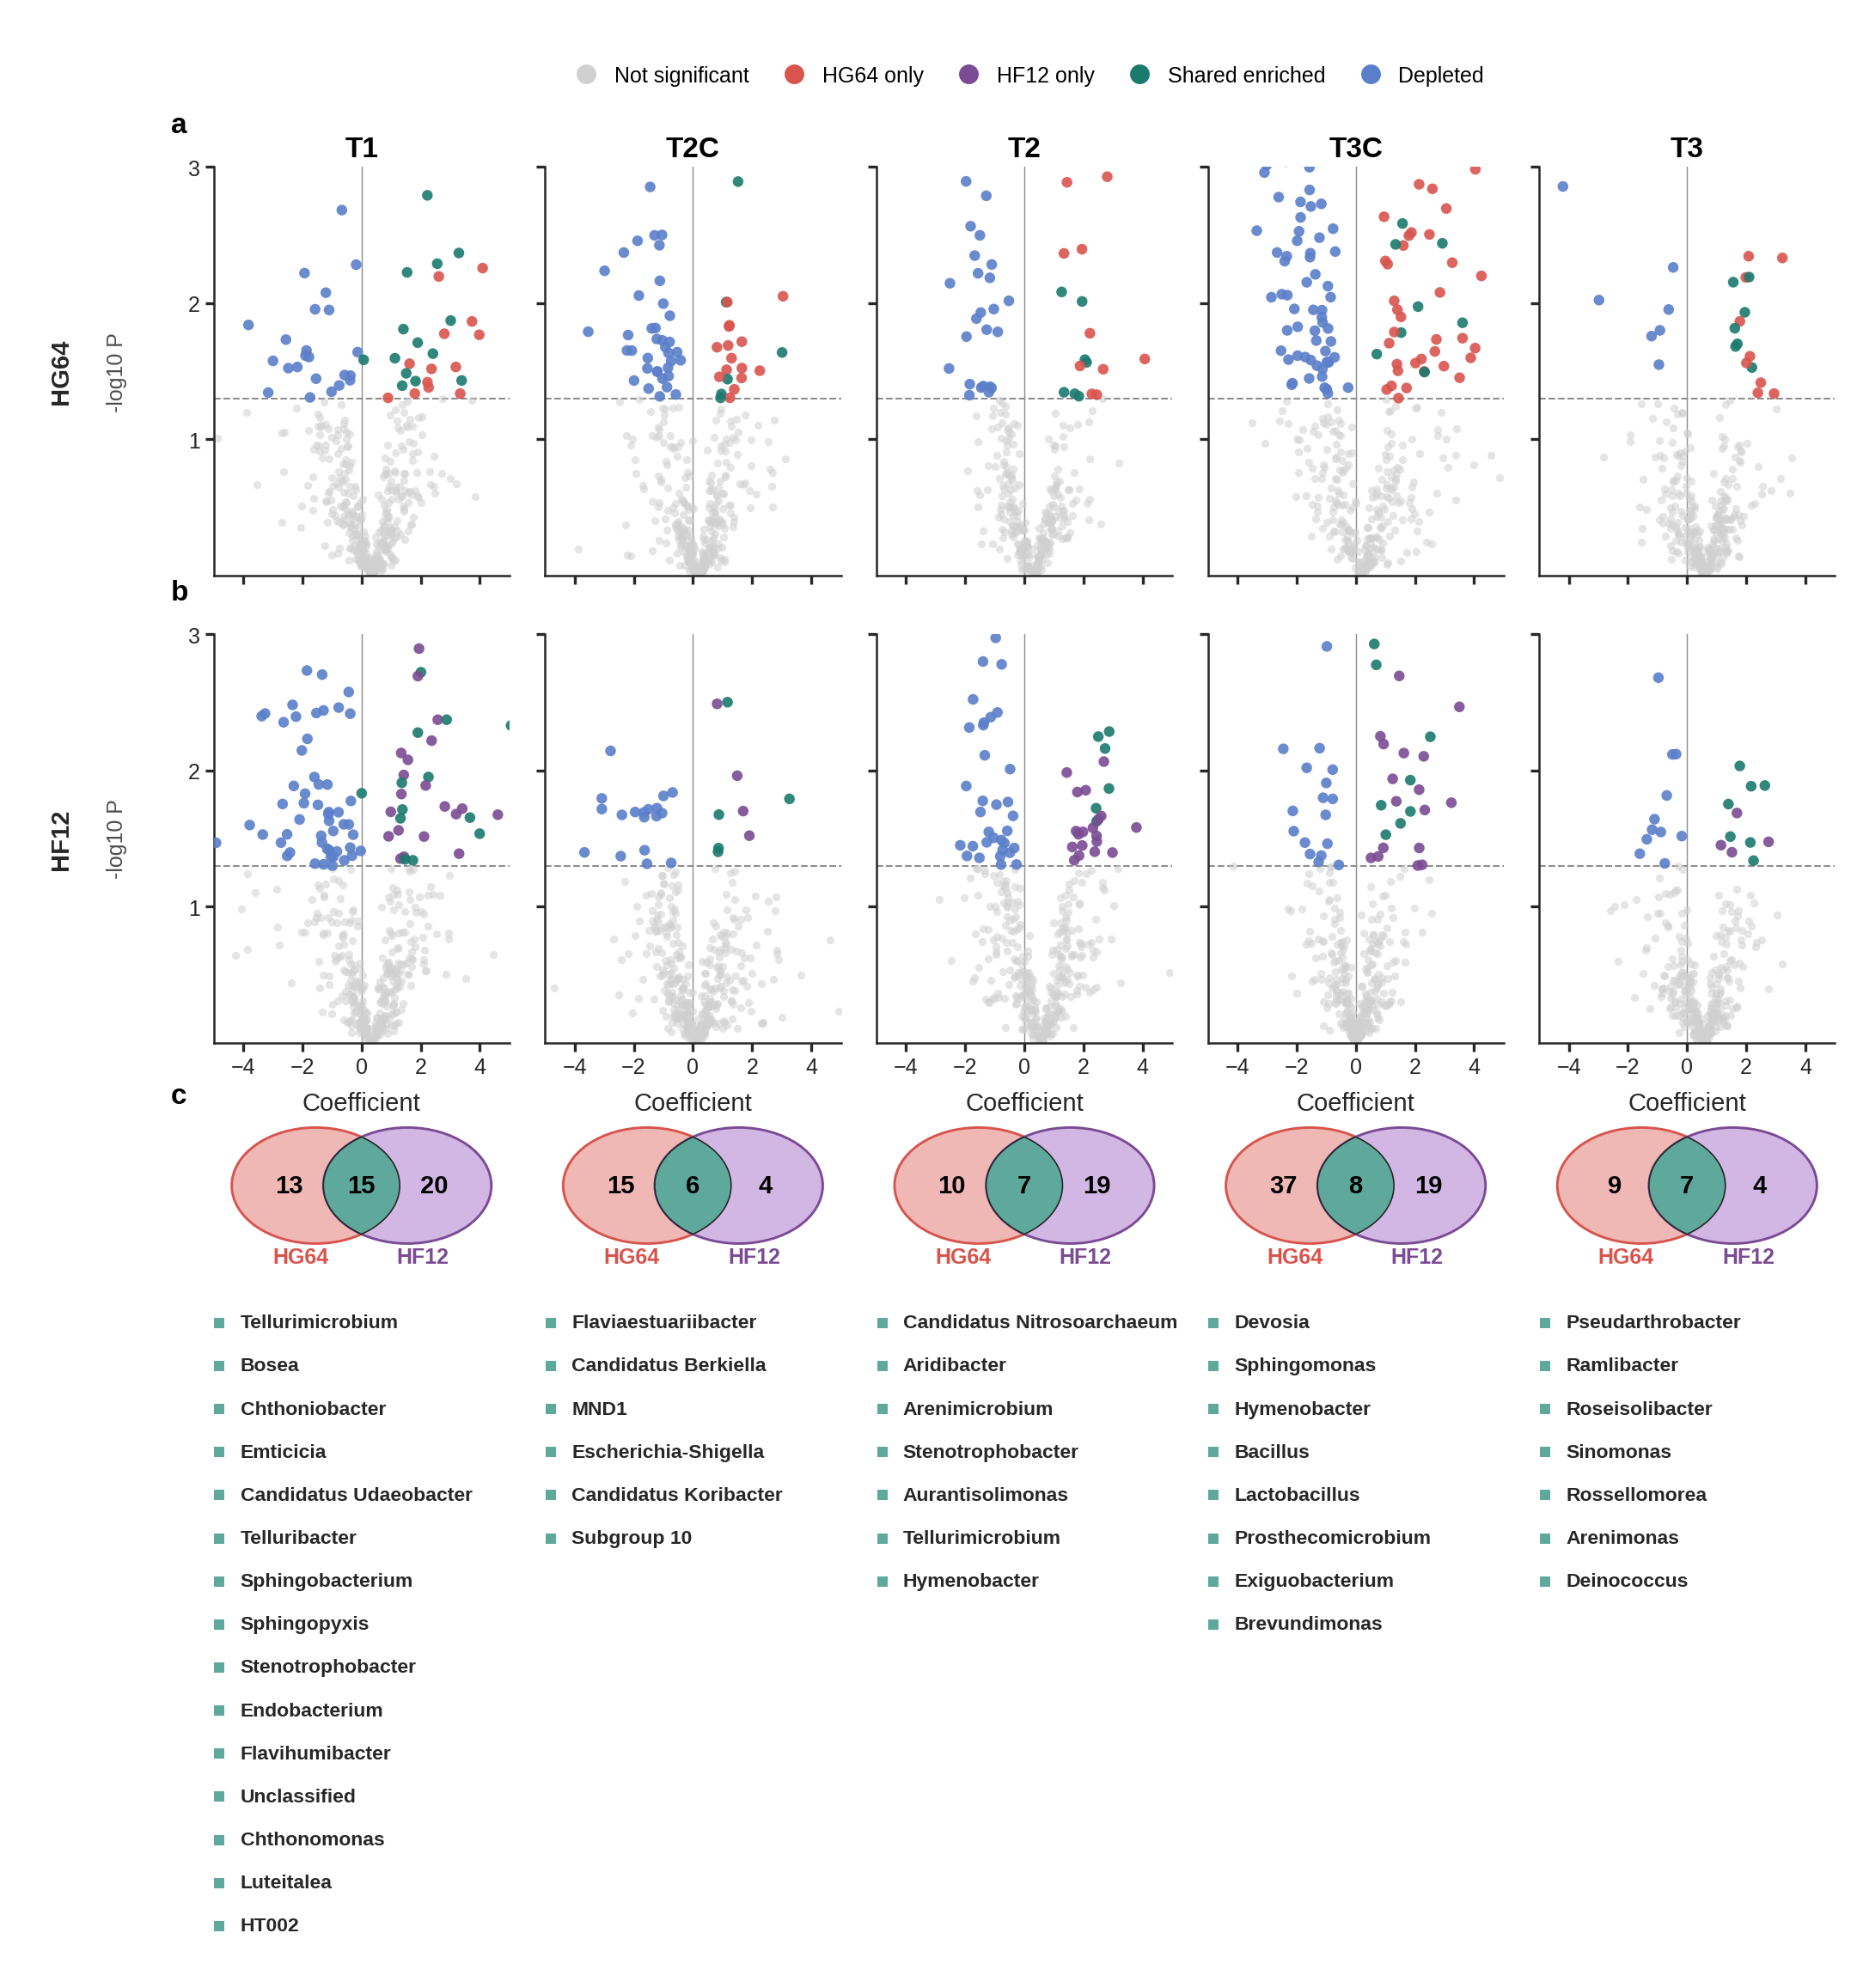
\includegraphics[width=0.94\linewidth]{Case-study-1-Fig2_16s_genus_enrichment.png}
  \caption{Differentially enriched genera in the resistant tomato parent HG64
    and progeny HF12.  MaAsLin~3 compared each resistant cultivar with pooled
    susceptible cultivars at each sampling point.  Shared enrichment denotes a
    positive coefficient and nominal $P<0.05$ in both contrasts.}
  \label{fig:tomato-enrichment}
\end{figure}

\FloatBarrier

% TODO: complete the release-specific evidence record for all comparison cells.
\begin{table}[htbp]
  \centering
  \caption{Reported capabilities of bioinformatics agents relevant to end-to-end
    microbiome analysis.  The three microbiome columns specifically
    concern analysis beginning with sequencing reads.}
  \label{tab:agent-capabilities}
  \scriptsize
  \setlength{\tabcolsep}{2.5pt}
  \renewcommand{\arraystretch}{1.25}
  \begin{tabularx}{\linewidth}{@{}l*{6}{>{\centering\arraybackslash}X}@{}}
    \toprule
      & \multicolumn{2}{c}{Agent operation}
      & \multicolumn{3}{c}{Microbiome analysis from reads}
      & Deployment \\
    \cmidrule(lr){2-3}\cmidrule(lr){4-6}\cmidrule(l){7-7}
    Agent
      & Autonomous workflow execution
      & Human-in-the-loop
      & 16S amplicon
      & Reference-based shotgun
      & Assembly / MAG
      & On-premises analysis \\
    \midrule
    BIA
      & $\checkmark$ & \textemdash & \textemdash & \textemdash & \textemdash & $\checkmark$ \\
    BioChatter
      & \textemdash & $\checkmark$ & \textemdash & \textemdash & \textemdash & $\checkmark$ \\
    AutoBA
      & $\checkmark$ & \textemdash & \textemdash & \textemdash & \textemdash & $\checkmark$ \\
    \shortstack[l]{Biomni\\(open-source)}
      & $\checkmark$ & \textemdash & \textemdash & \textemdash & \textemdash & $\checkmark$ \\
    BioAgents
      & \textemdash & \textemdash & \textemdash & \textemdash & \textemdash & \textemdash \\
    M3A
      & $\checkmark$ & $\checkmark$ & \textemdash & \textemdash & \textemdash & $\checkmark$ \\
    BioMedAgent
      & $\checkmark$ & \textemdash & \textemdash & \textemdash & \textemdash & $\checkmark$ \\
    BioMaster
      & $\checkmark$ & \textemdash & \textemdash & $\checkmark$ & \textemdash & $\checkmark$ \\
    MetaClaw
      & $\checkmark$ & \textemdash & $\checkmark$ & $\checkmark$ & $\checkmark$ & $\checkmark$(partial) \\
    MicroBioAgent
      & $\checkmark$ & $\checkmark$ & $\checkmark$ & $\checkmark$ & $\checkmark$ & $\checkmark$ \\
    \bottomrule
  \end{tabularx}
  \vspace{0.35em}

  \begin{minipage}{\linewidth}
    \footnotesize
    \textit{Notes:} $\checkmark$, reported support,
    \textemdash, support not established from the reviewed sources, which
    does not demonstrate inability. The comparison draws on the published
    descriptions of the related systems
    \parencite{zhou2024autoba,huang2025biomni,mehandru2025bioagents,
    johri2026m3a,xin2024bia,lobentanzer2025biochatter,
    bu2026biomedagent,su2026biomaster,zhang2026metaclaw}.
    Biomni denotes the open-source release.
    MetaClaw reports assembly and genome-resolved binning through FlowHub
    \parencite{zhang2026metaclaw}. Its partial on-premises designation reflects
    the use of FlowHub for upstream metagenomic processing and local containers
    for downstream analysis.     This scope comparison is not a performance benchmark.
  \end{minipage}
\end{table}

\begin{table}[htbp]
  \centering
  \caption{Differential-abundance methods and replicates averaged in the
    detailed-versus-medium prompt comparison.  Each row is one comparison.
    Session counts are the replicates, out of three, whose result for that
    method entered the average.}
  \label{tab:da-prompt-methods}
  \scriptsize
  \setlength{\tabcolsep}{4pt}
  \renewcommand{\arraystretch}{1.18}
  \begin{tabular}{@{}llccc@{}}
    \toprule
    Model & Method
      & \shortstack{Detailed\\sessions}
      & \shortstack{Medium\\sessions}
      & \shortstack{Taxa\\compared} \\
    \midrule
    \multicolumn{5}{@{}l}{\textit{16S rRNA gene, genus}} \\
    \addlinespace
    DeepSeek-Pro   & DESeq2            & 1/3 & 1/3 & 111 \\
    DeepSeek-Flash & DESeq2            & 2/3 & 2/3 & 668 \\
    GLM-Flash      & DESeq2            & 3/3 & 1/3 & 413 \\
    \addlinespace
    \multicolumn{5}{@{}l}{\textit{Shotgun metagenome, species}} \\
    \addlinespace
    DeepSeek-Pro   & Wilcoxon          & 1/3 & 1/3 & 14 \\
    DeepSeek-Flash & Mann--Whitney $U$ & 1/3 & 1/3 & 39 \\
    GLM-Flash      & DESeq2            & 2/3 & 1/3 & 9 \\
    \bottomrule
  \end{tabular}
  \vspace{0.35em}

  \begin{minipage}{\linewidth}
    \footnotesize
    \textit{Notes:} The simple prompt was not included.  Display names
    correspond to \texttt{deepseek-v4-pro}, \texttt{deepseek-v4-flash}, and
    \texttt{glm5.3-flash}.  Within a replicate, the median log$_2$ fold change
    of each taxon was retained.  Those values were then averaged across the
    included replicates; a taxon missing from a replicate was not imputed as
    zero.  A taxon was compared only when both prompts produced a finite
    value.  DESeq2 values are negative-binomial log$_2$ fold changes.
    Wilcoxon and Mann--Whitney $U$ values are log$_2$ ratios of group means
    reported with the rank test, not the rank statistic.  One DeepSeek-Flash
    detailed replicate reported only ASV-level DESeq2 results and was excluded
    from the genus comparison.  One GLM-Flash detailed replicate did not
    analyse shotgun libraries.
  \end{minipage}
\end{table}

\begin{table}[htbp]
  \centering
  \caption{DESeq2 sessions included in the cross-model comparison of
    differential-abundance effect sizes.  Each row is one model.  Session
    counts are the replicates, out of three, whose DESeq2 result entered the
    comparison.  The medium shotgun prompt produced no DESeq2 results.}
  \label{tab:da-model-methods}
  \scriptsize
  \setlength{\tabcolsep}{4pt}
  \renewcommand{\arraystretch}{1.18}
  \begin{tabular}{@{}lcccc@{}}
    \toprule
    Model
      & \shortstack{Detailed\\sessions}
      & \shortstack{Medium\\sessions}
      & \shortstack{Detailed\\taxa shared}
      & \shortstack{Medium\\taxa shared} \\
    \midrule
    \multicolumn{5}{@{}l}{\textit{16S rRNA gene, genus}} \\
    \addlinespace
    DeepSeek-Pro   & 1/3 & 1/3 & 216 & 332 \\
    DeepSeek-Flash & 2/3 & 2/3 & 216 & 332 \\
    GLM-Flash      & 3/3 & 1/3 & 216 & 332 \\
    \addlinespace
    \multicolumn{5}{@{}l}{\textit{Shotgun metagenome, species}} \\
    \addlinespace
    DeepSeek-Pro   & 1/3 & \textemdash & 43 & \textemdash \\
    DeepSeek-Flash & 2/3 & \textemdash & 43 & \textemdash \\
    GLM-Flash      & 2/3 & \textemdash & 43 & \textemdash \\
    \bottomrule
  \end{tabular}
  \vspace{0.35em}

  \begin{minipage}{\linewidth}
    \footnotesize
    \textit{Notes:} Display names correspond to \texttt{deepseek-v4-pro},
    \texttt{deepseek-v4-flash} and \texttt{glm5.3-flash}.  A taxon was
    shared when every included session reported a finite DESeq2 log$_2$ fold
    change for it, so the shared count is the same in each row of a block.
    Within a session, the value for a taxon is that session's DESeq2
    coefficient; values were then averaged across the included sessions.
    One GLM-Flash detailed replicate did not analyse shotgun libraries.
  \end{minipage}
\end{table}

\begin{figure}[htbp]
  \centering
  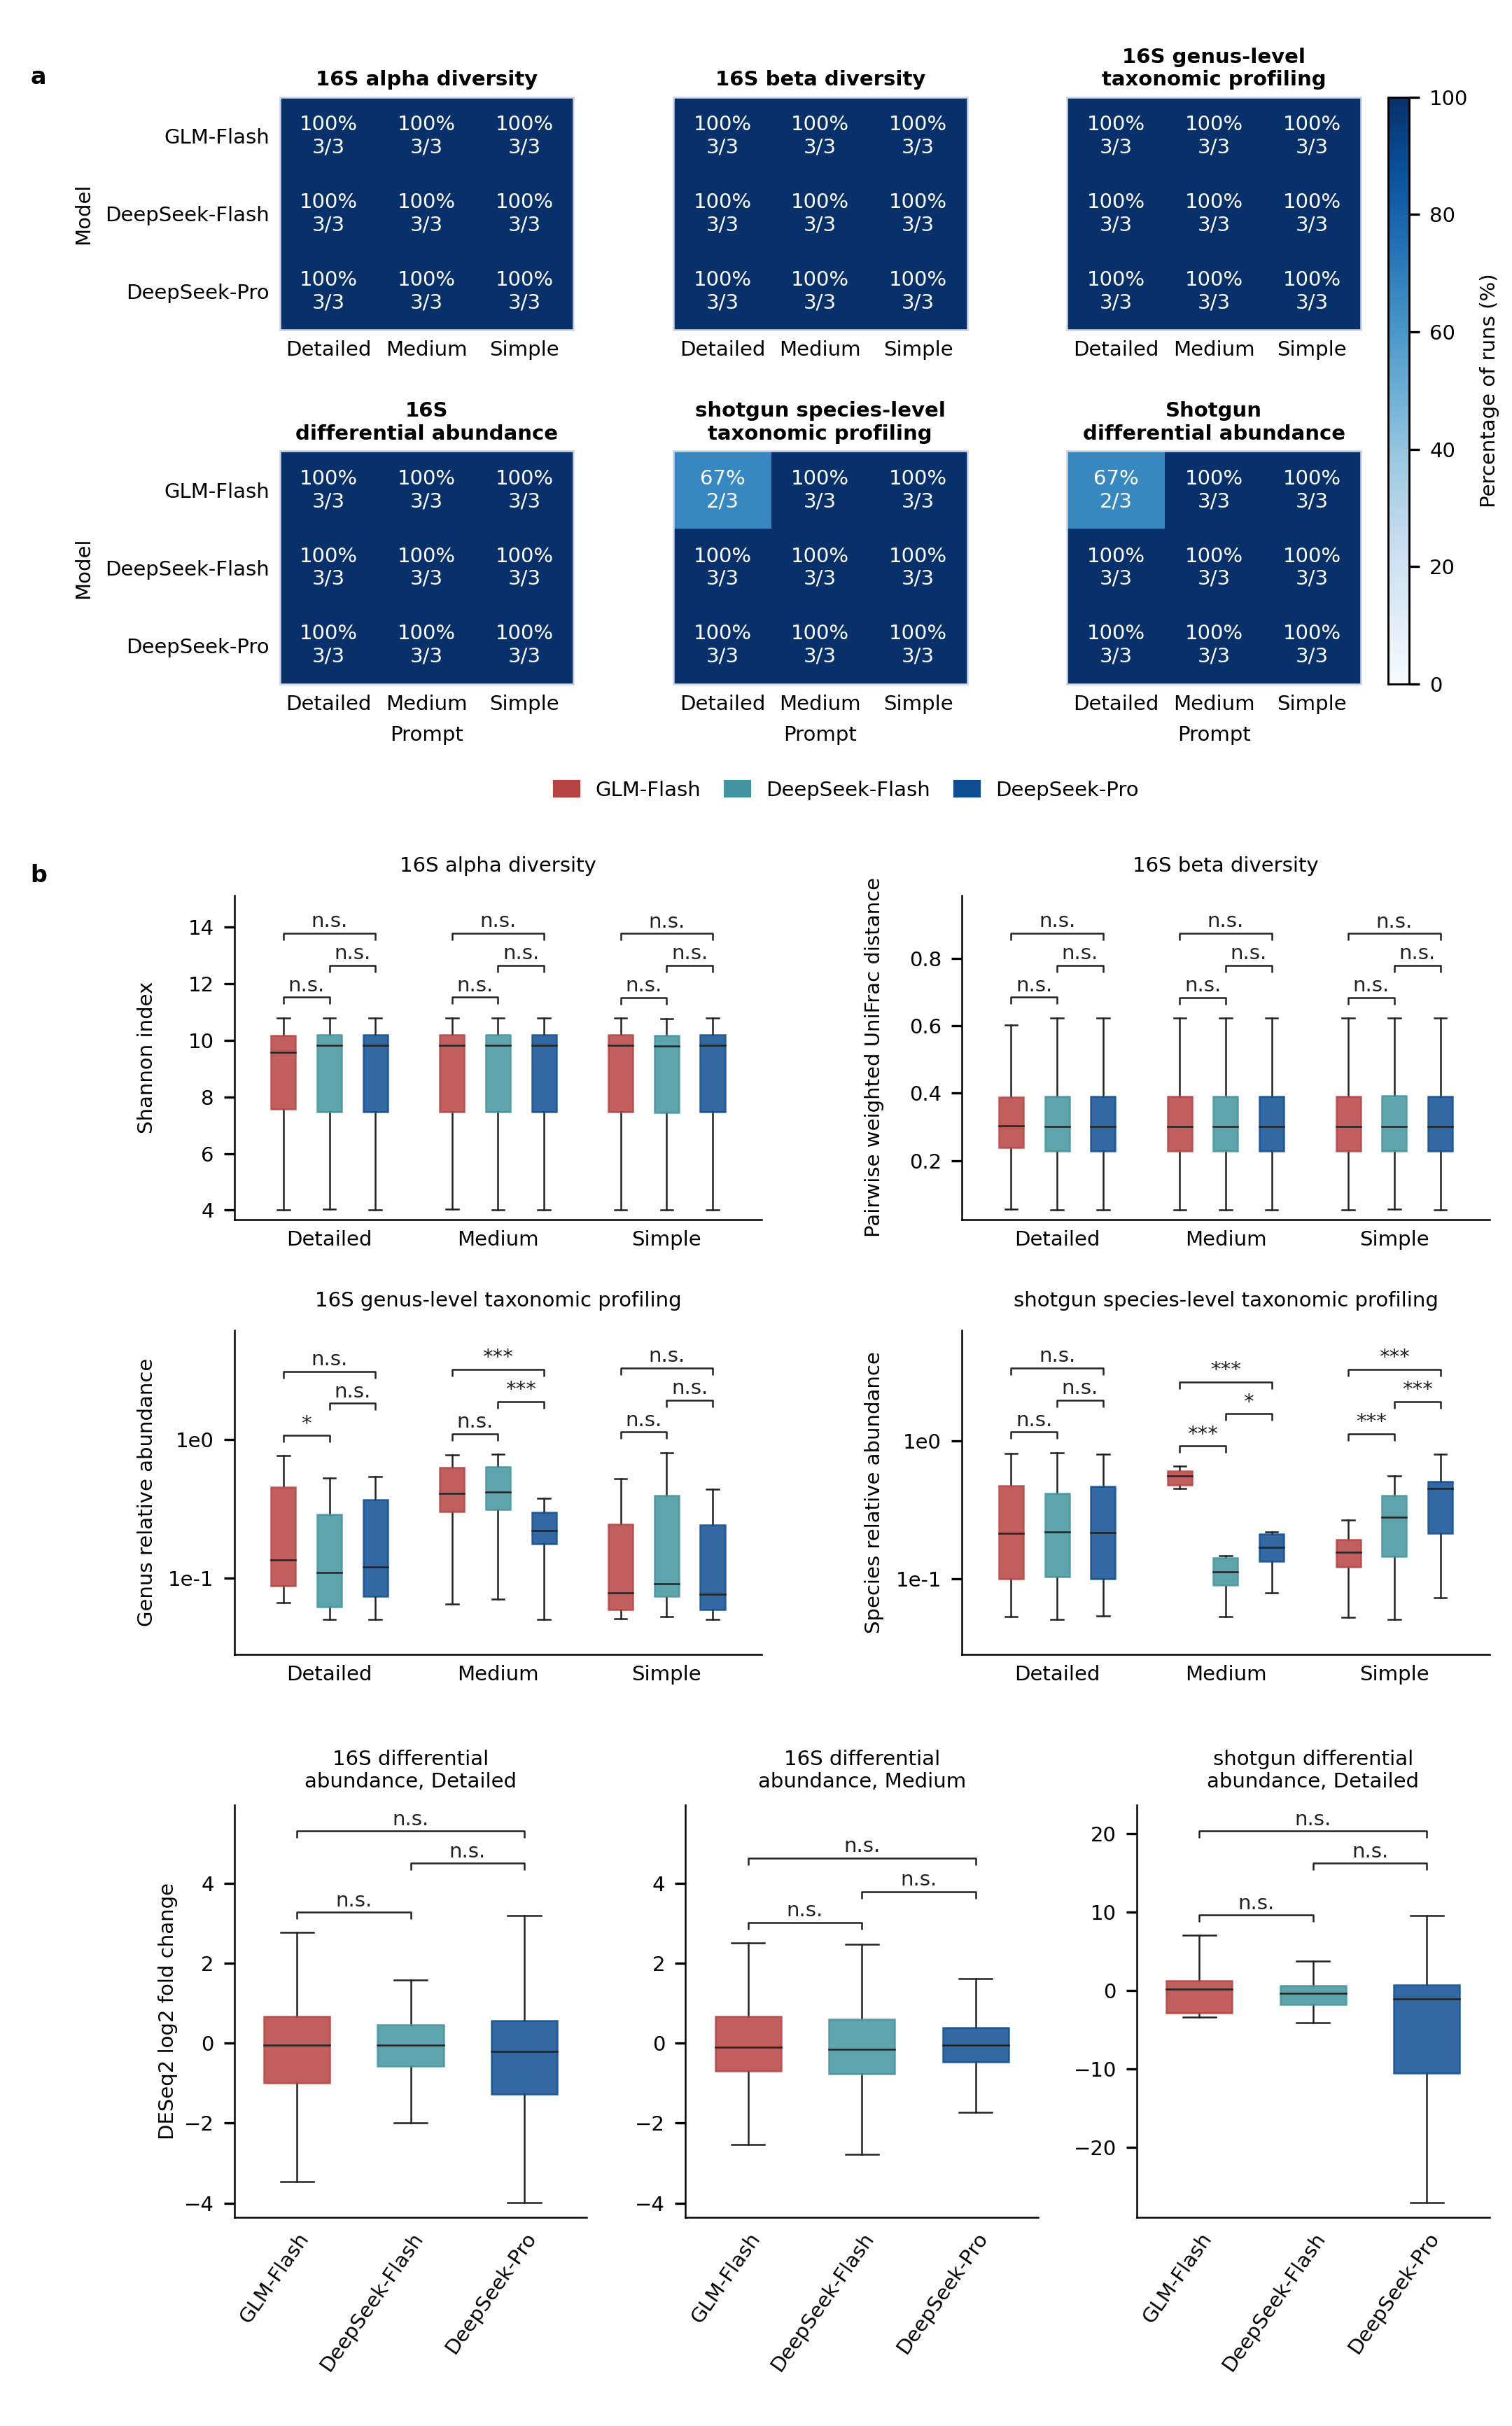
\includegraphics[width=\linewidth]{case1_completion_models.png}
  \caption{Task completion and cross-model comparisons on the frozen Case~1
    inputs.  (a)~Completion of six requested analyses.  Each cell is the
    number of sessions, out of three, in which the analysis was completed.
    The GLM-Flash detailed shotgun cells are 2/3 because one session
    contained no shotgun reads.  (b)~Shannon index, pairwise weighted
    UniFrac distance, relative abundance and DESeq2 log$_2$ fold change
    compared among models within each prompt.  Shannon points are
    session means of per-sample indexes.  UniFrac points are session means
    of distances between unordered sample pairs ($n = 1{,}770$).
    Relative-abundance points are session means for taxa whose mean was at
    least 5\% in every compared group.  DESeq2 points are means across
    sessions that ran DESeq2, for taxa shared by the compared models
    (Supplementary Table~\ref{tab:da-model-methods}); the medium shotgun
    prompt had no such sessions.  Brackets are two-sided Mann--Whitney $U$
    tests with Holm correction within each set of three pairs.  n.s.,
    Holm-adjusted $P \geq 0.05$; *, $P < 0.05$; **, $P < 0.01$; ***,
    $P < 0.001$.  Samples, sample pairs and taxa come from one experiment
    and are not independent replicates.}
  \label{fig:robustness-models}
\end{figure}

\begin{figure}[htbp]
  \centering
  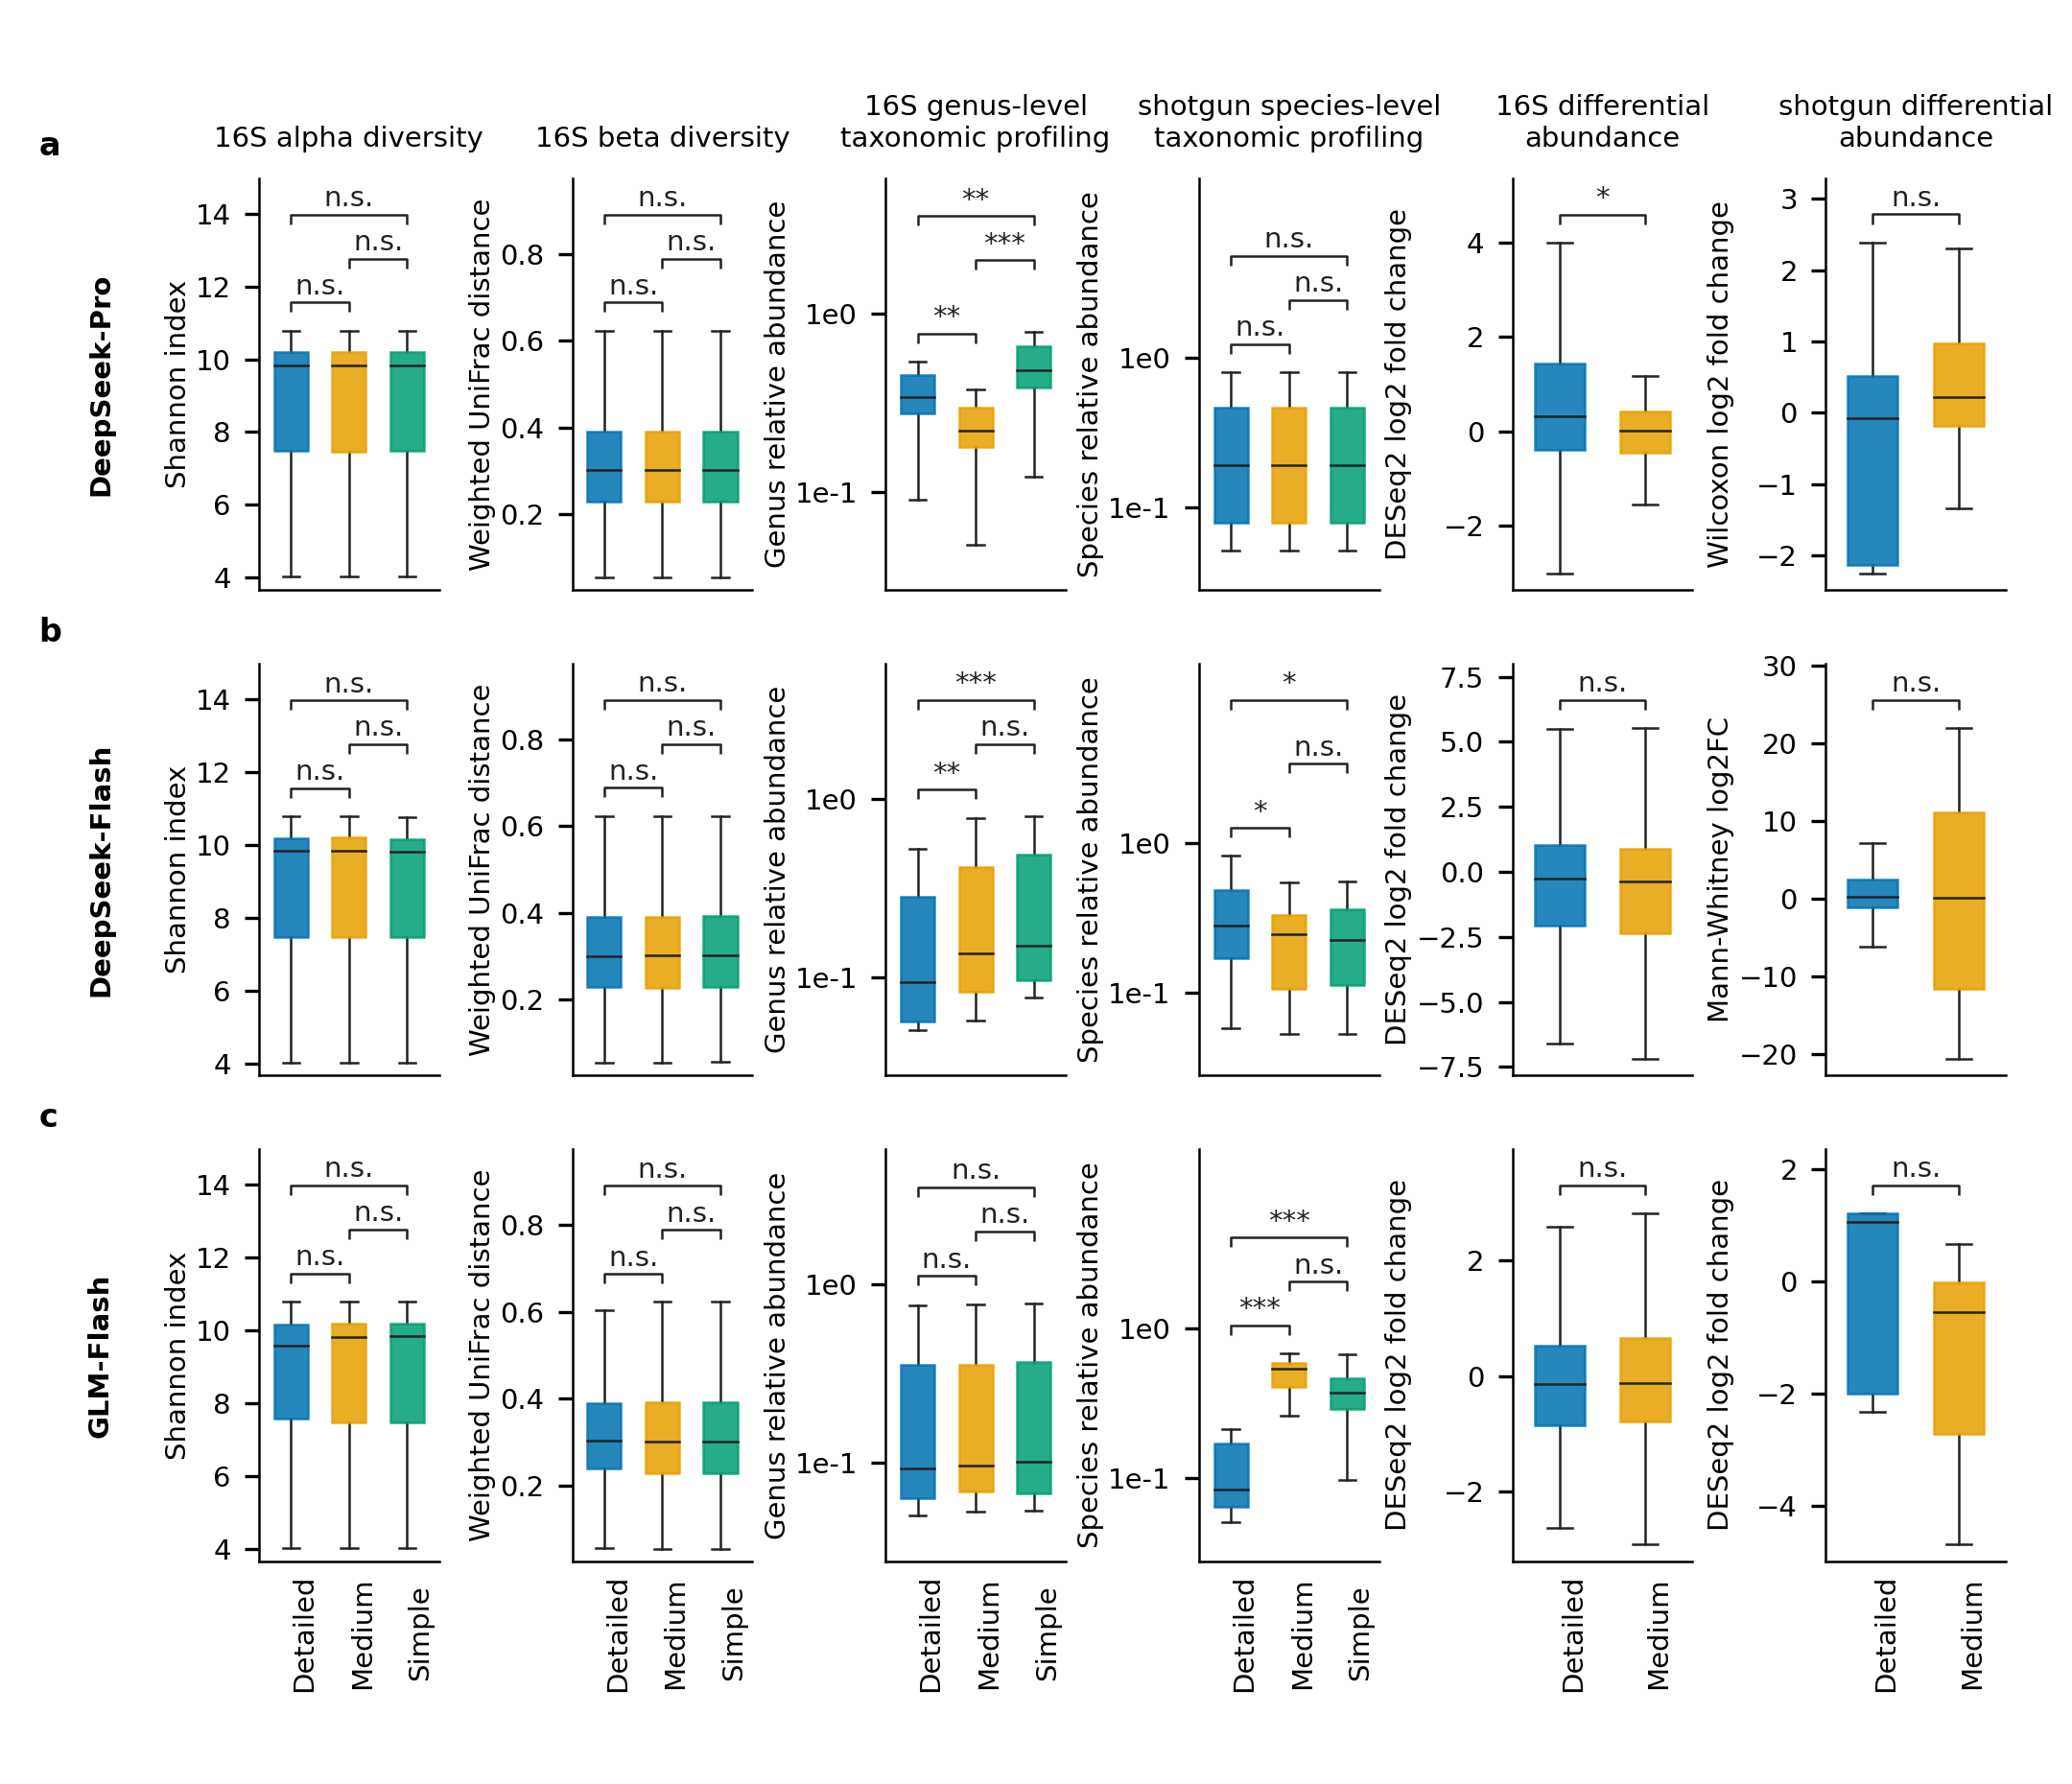
\includegraphics[width=\linewidth]{by_prompt_models.png}
  \caption{Within-model comparisons across prompt levels.  Rows are
    DeepSeek-Pro, DeepSeek-Flash and GLM-Flash.  The first four columns
    follow the point definitions in Supplementary
    Figure~\ref{fig:robustness-models}.  The differential-abundance columns
    compare the detailed and medium prompts only.  16S values are DESeq2
    log$_2$ fold changes.  Shotgun values are Wilcoxon, Mann--Whitney $U$
    and DESeq2 log$_2$ fold changes for DeepSeek-Pro, DeepSeek-Flash and
    GLM-Flash, respectively (Supplementary Table~\ref{tab:da-prompt-methods}),
    and are not compared across rows.  Brackets in the first four columns
    are two-sided Mann--Whitney $U$ tests with Holm correction within each
    set of three prompt pairs.  Each differential-abundance bracket is a
    single pair.  n.s., adjusted $P \geq 0.05$; *, $P < 0.05$; **,
    $P < 0.01$; ***, $P < 0.001$.  Samples, sample pairs and taxa come from
    one experiment and are not independent replicates.}
  \label{fig:robustness-prompts}
\end{figure}

\FloatBarrier

\end{document}
